\documentclass[aspectratio=169,10pt]{beamer}
\usetheme{default}
\usecolortheme{seahorse}
\setbeamertemplate{navigation symbols}{}
\setbeamertemplate{footline}[frame number]
\usepackage{graphicx, booktabs}
\graphicspath{{../figures/}}
\title{Run 224489: Wiring Fix Confirmed, First Plastic-MIP Calibration\\
       from LIQ Triples, and HV Scan 2}
\subtitle{n\_TOF EAR2 X17 --- first run with the liquid scintillators (July 17, 2026)}
\author{Dylan Neff \\[0.5ex] {\small analysis and slides prepared with Claude (Anthropic AI assistant)}}
\date{July 18, 2026}

\begin{document}

\begin{frame}\titlepage\end{frame}

\begin{frame}{Run 224489: what changed since the last scan (224466)}
\begin{columns}
\column{.55\textwidth}
\begin{itemize}
\item \textbf{Cabling fix} on the crossed A/D channels.
\item \textbf{FIFO}: plastics on a linear fan-in/fan-out instead of the
      BNC-T split ($\sim$16 ns extra delay, naive $2\times$ amplitude).
\item \textbf{Liquid scintillators} (LIQA--D, 1 ch/arm) in the readout for
      the first time: 5.3 M (C) -- 21.6 M (B) hits.
\item SiPM flash gating \textbf{ON all run} (no boundary).
\item Same 9-step plastic HV ladder, 1200--1600 V in 50 V merged grid,
      + post-scan nominal-HV window.
\end{itemize}
\column{.42\textwidth}
\begin{itemize}
\item 1750 bunches (817 dedicated), new PSA with LIQ pulse-shape fitting.
\item QA clean: \textbf{no wall outage} (0/1750; 224404 lost 46\%),
      $\gamma$-flash 11.62 $\mu$s on all arms, all 44 channels alive.
\end{itemize}
\end{columns}
\end{frame}

\begin{frame}{Scan timeline: bunches $\to$ HV steps via the CAEN log}
\centering
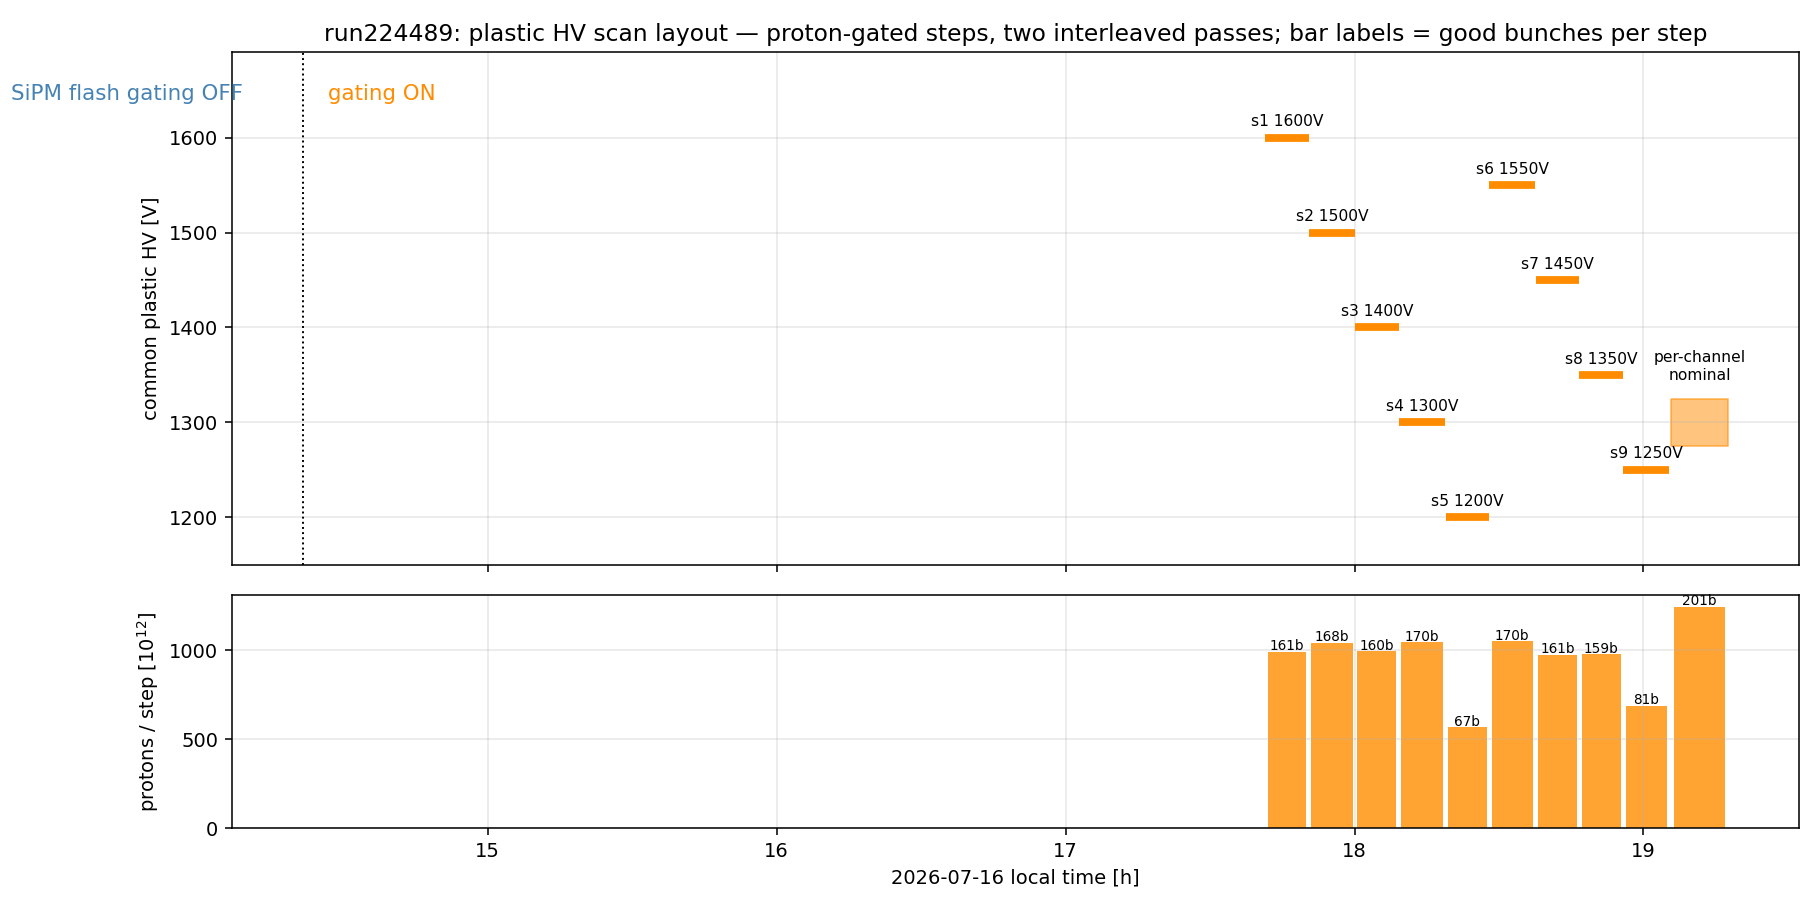
\includegraphics[width=\textwidth,height=.8\textheight,keepaspectratio]{12_hv_scan/scan_timeline.png}
\end{frame}

\begin{frame}{Result 1 --- the cross-wiring fix is \textbf{confirmed}; A/D closed}
\begin{itemize}
\item Duplication band ($\pm$4 ns equal-amplitude partner, one group over):
      flagged fractions were \alert{23--31\%} on the crossed A/D channels in
      224460 $\to$ now $\leq$4\% everywhere = B-arm control level.
\item Wall--plastic excess now \textbf{equal on all four arms}
      (1.71--1.81 M within $\pm$10 ns) --- was 6--8$\times$ deficient on A/D.
\item A/D coincident wall spectra show clean MIP bumps with \textbf{no veto}.
\end{itemize}
\centering
\alert{The standing A/D coincidence deficit was the cabling. Closed.}
\end{frame}

\begin{frame}{A/D duplication autopsy: before-and-after}
\centering

\includegraphics[width=\textwidth,height=.78\textheight,keepaspectratio]{run224489/autopsy/dup_veto_spectra.png}
\end{frame}

\begin{frame}{HV scan: wall MIP again immune to plastic HV (now incl.\ arm A)}
\centering
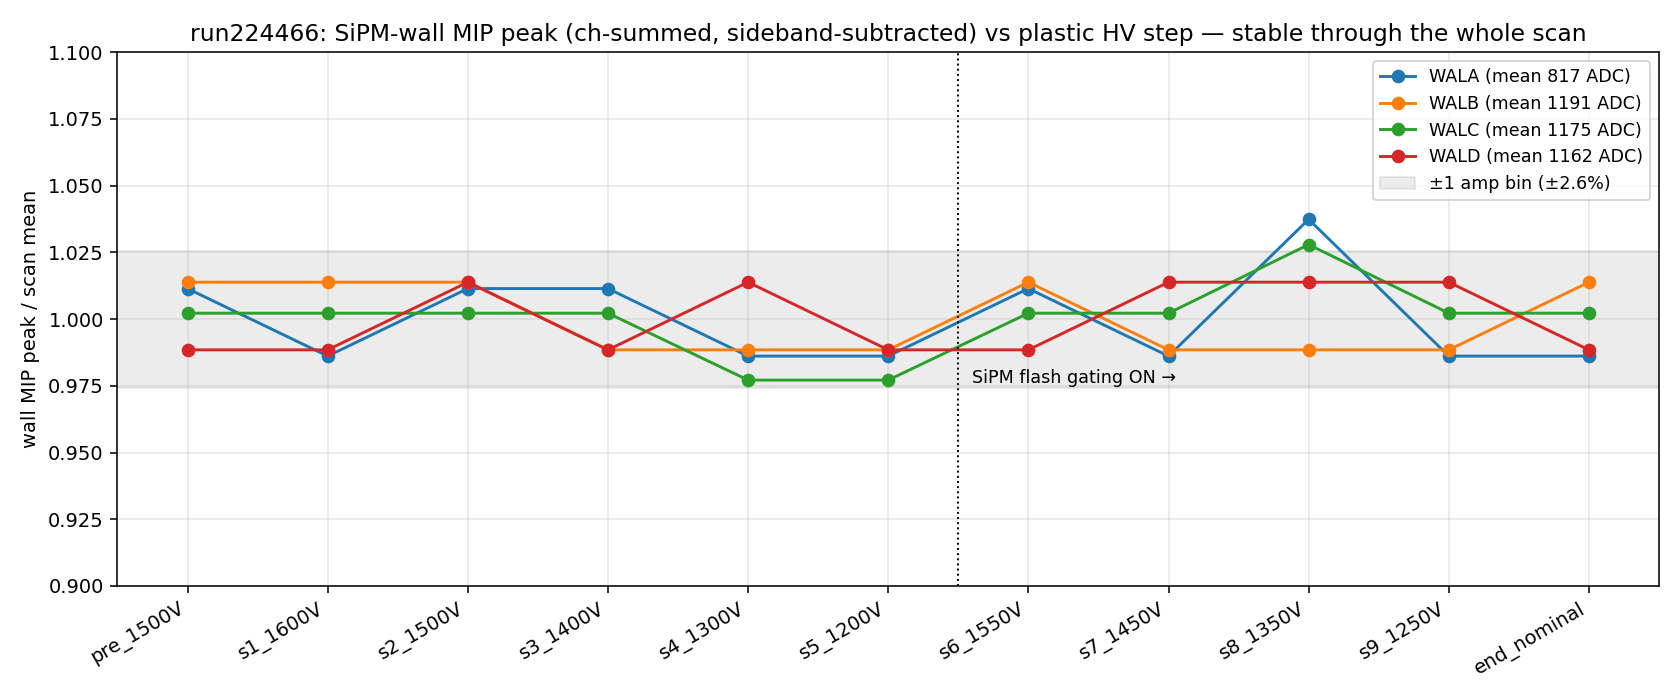
\includegraphics[width=\textwidth,height=.72\textheight,keepaspectratio]{12_hv_scan/wall_mip_stability.png}

{\small $\pm$1 bin ($\pm$2.6\%) over a $3\times$ tag-rate change $\Rightarrow$
wall energy scale independent of plastic operating point.}
\end{frame}

\begin{frame}{Per-PMT gain power laws $G\propto V^{n}$, $n=3.8$--$7.1$}
\centering
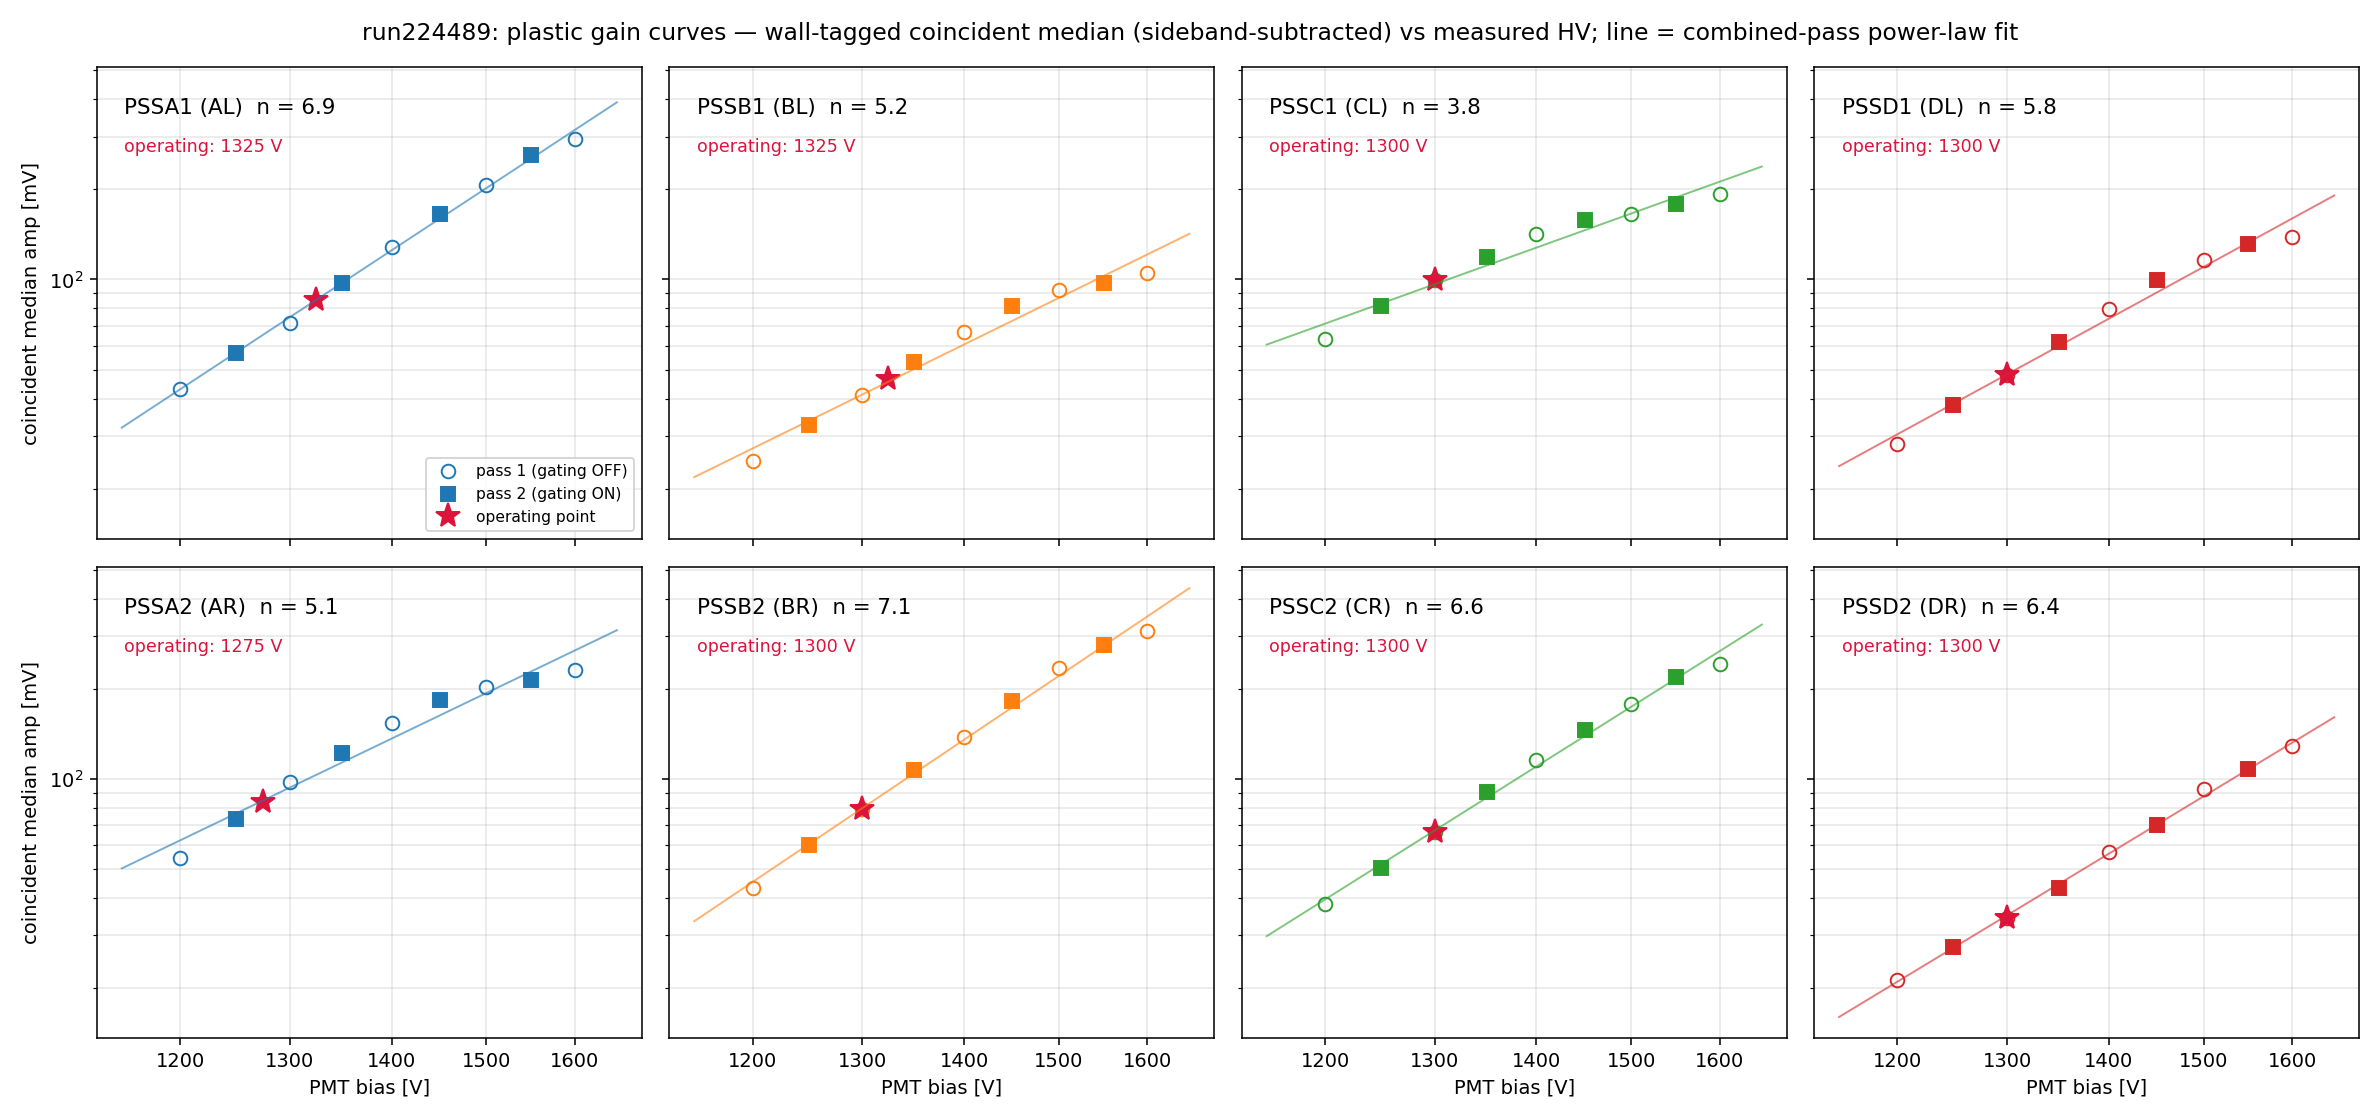
\includegraphics[width=\textwidth,height=.78\textheight,keepaspectratio]{12_hv_scan/gain_curves.png}
\end{frame}

\begin{frame}{Result 2 --- the FIFO gain ratio is \textbf{1.4}, not 2}
\centering
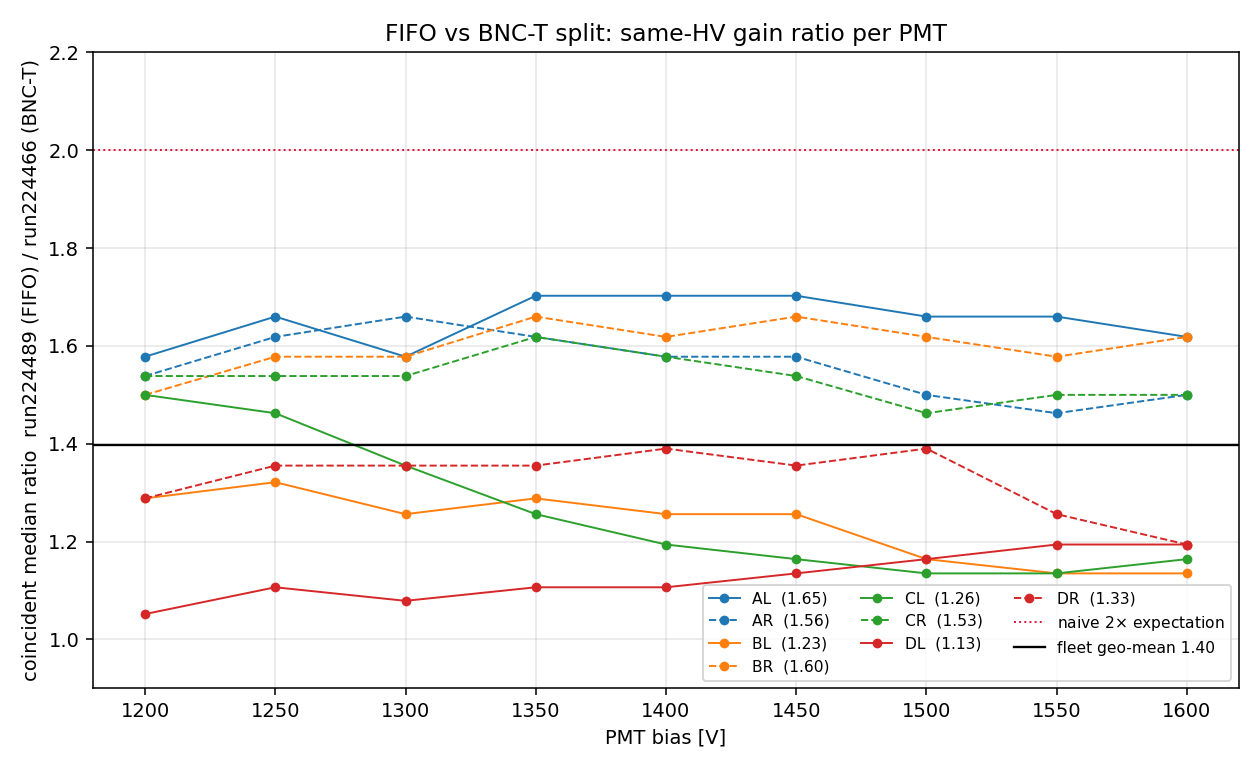
\includegraphics[width=\textwidth,height=.68\textheight,keepaspectratio]{19_triples/fifo_ratio.png}

{\small Same-HV coincident medians, 224489/224466: fleet geo-mean $\times$1.40,
per-PMT 1.13 (DL) -- 1.65 (AL). Use the measured per-PMT ratios, not a global 2.}
\end{frame}

\begin{frame}{New HV equalization (supersedes 224466 table)}
\begin{columns}
\column{.5\textwidth}
\centering\small
\begin{tabular}{lrrr}
\toprule
PMT & med [mV] & $V_{\rm sugg}$ & $\Delta V$\\
\midrule
AL & 85.4 & 1271 & $-54$\\
AR & 83.6 & 1211 & $-64$\\
BL & 46.7 & 1409 & $+84$\\
BR & 79.2 & 1262 & $-38$\\
CL & 99.8 & 1158 & $-142$\\
CR & 66.5 & 1293 & $-7$\\
DL & 47.8 & 1368 & $+68$\\
DR & 34.4 & 1433 & $+133$\\
\bottomrule
\end{tabular}
\column{.47\textwidth}
\begin{itemize}
\item Target: fleet geo-mean coincident median (64.2 mV); spread now
      $2.9\times$.
\item At equalized gains: common threshold with 99\% tagged efficiency on
      every PMT down to \textbf{4.9 mV} (95\%: 7.1 mV).
\item Exported to DAQ repo (\texttt{calibrations/pss/, pss\_trigger/}).
\end{itemize}
\end{columns}
\end{frame}

\begin{frame}{Result 3 --- the liquids are timed in (first time)}
\centering
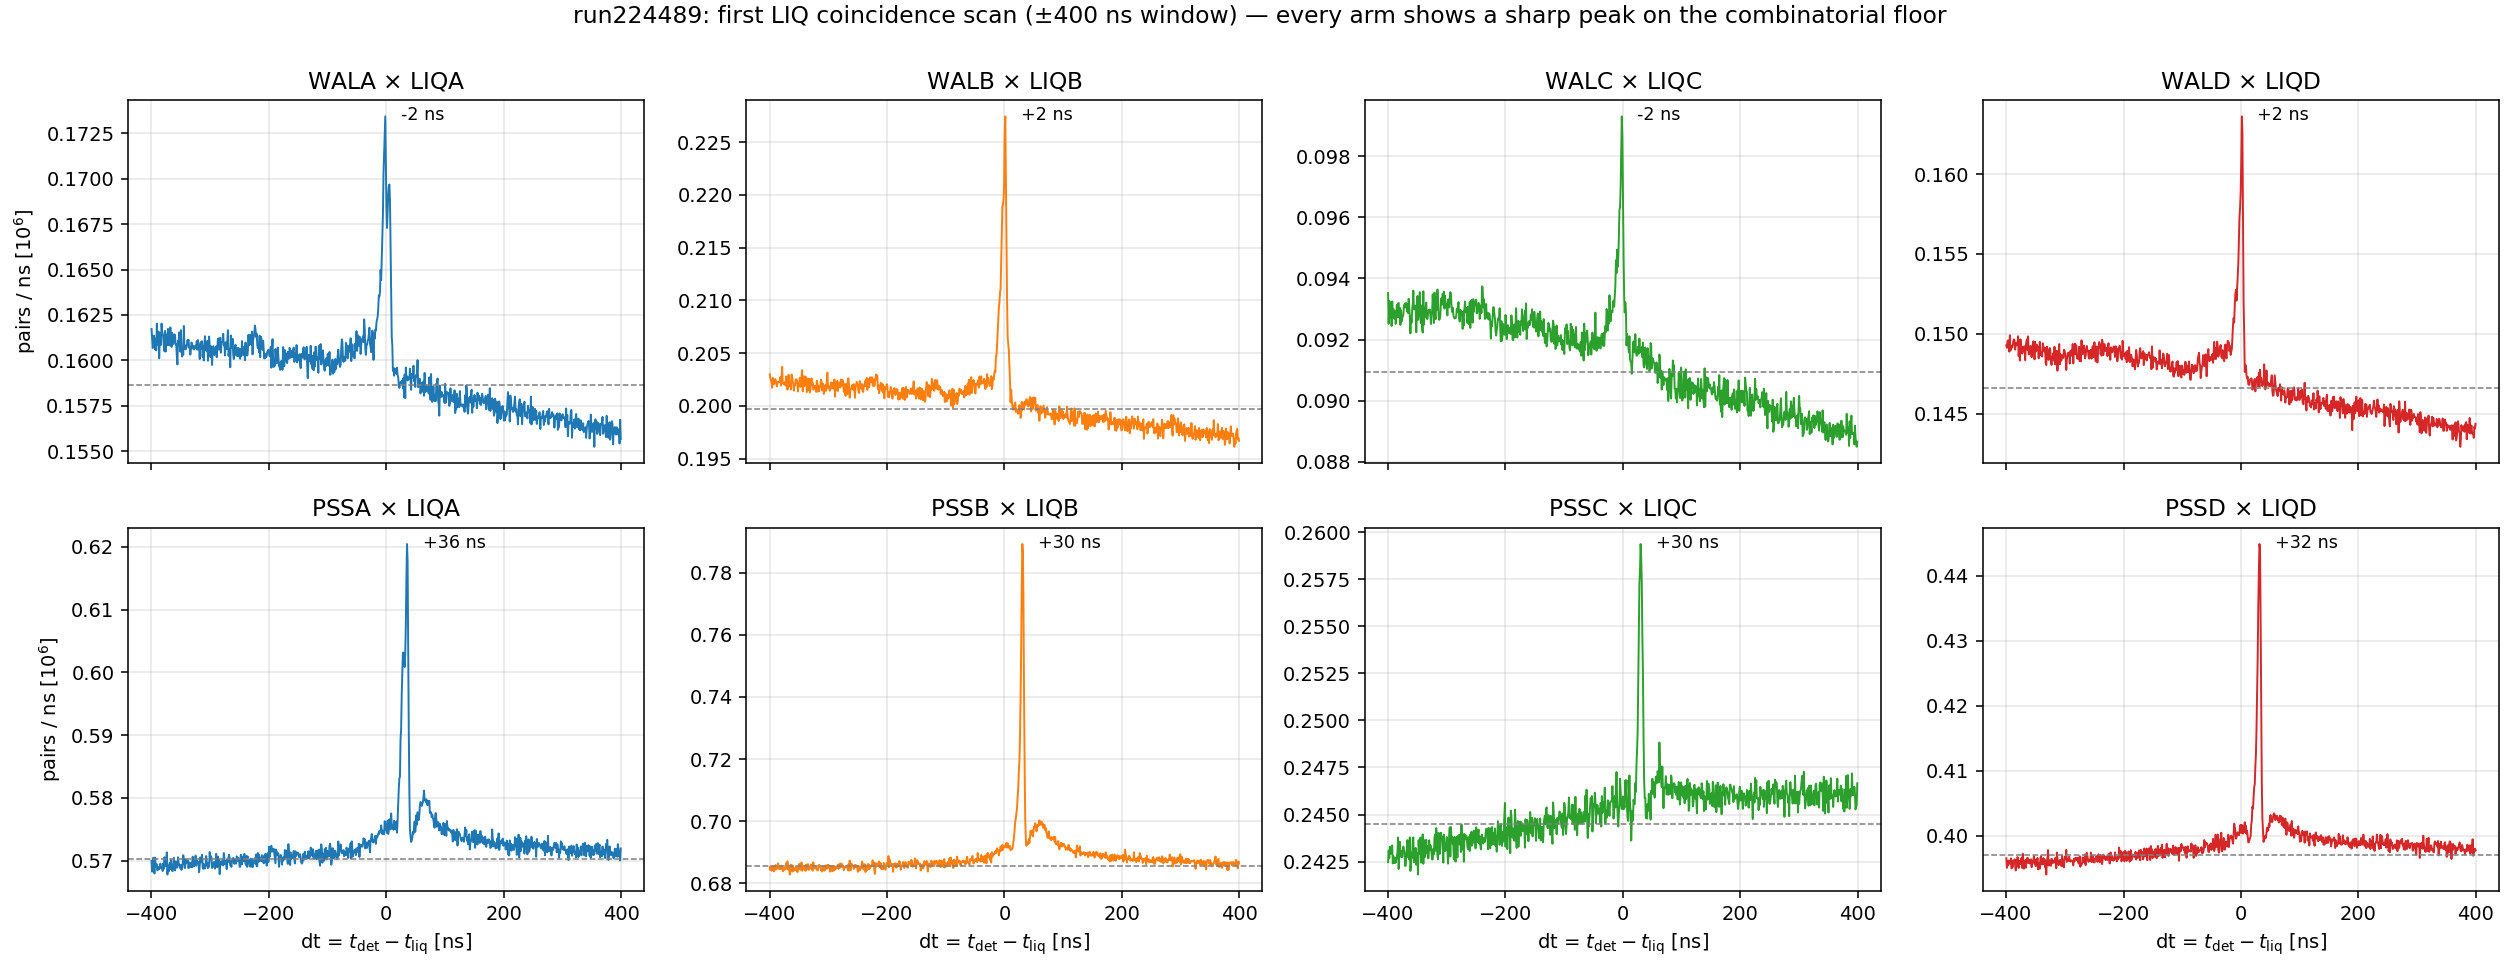
\includegraphics[width=\textwidth,height=.7\textheight,keepaspectratio]{19_triples/liq_wide_dt.png}

{\small LIQ leads the plastic by 29.5--32.8 ns, within $\pm$3.3 ns of the wall;
per-channel offsets (rms 3.2--4.5 ns) $\to$ \texttt{calib/liq\_offsets\_run224489.json}.}
\end{frame}

\begin{frame}{LIQ timing per wall channel / plastic bar}
\centering
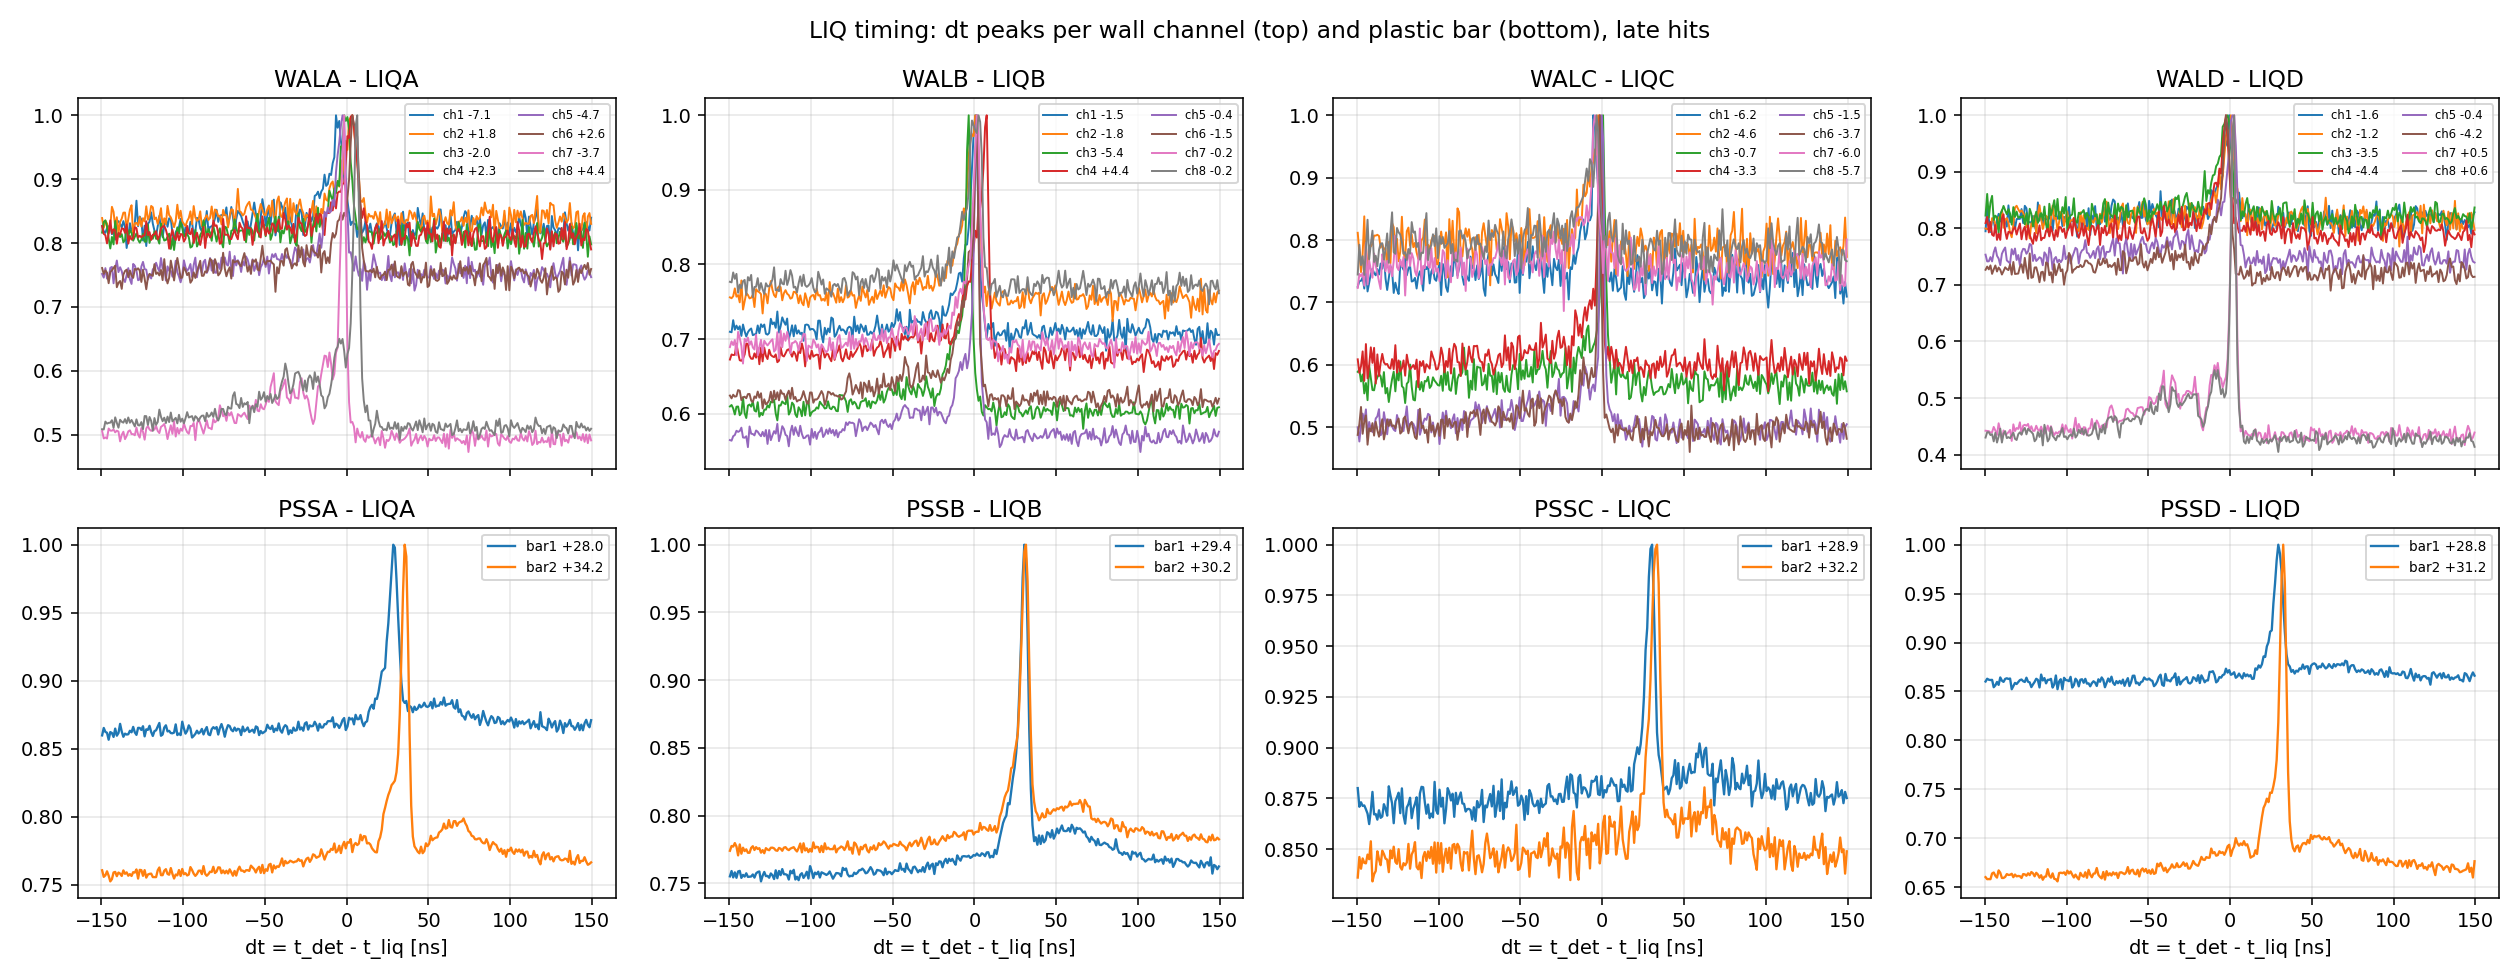
\includegraphics[width=\textwidth,height=.8\textheight,keepaspectratio]{19_triples/liq_timing.png}
\end{frame}

\begin{frame}{The triple telescope: why LIQ unlocks the \emph{plastic} MIP}
\centering
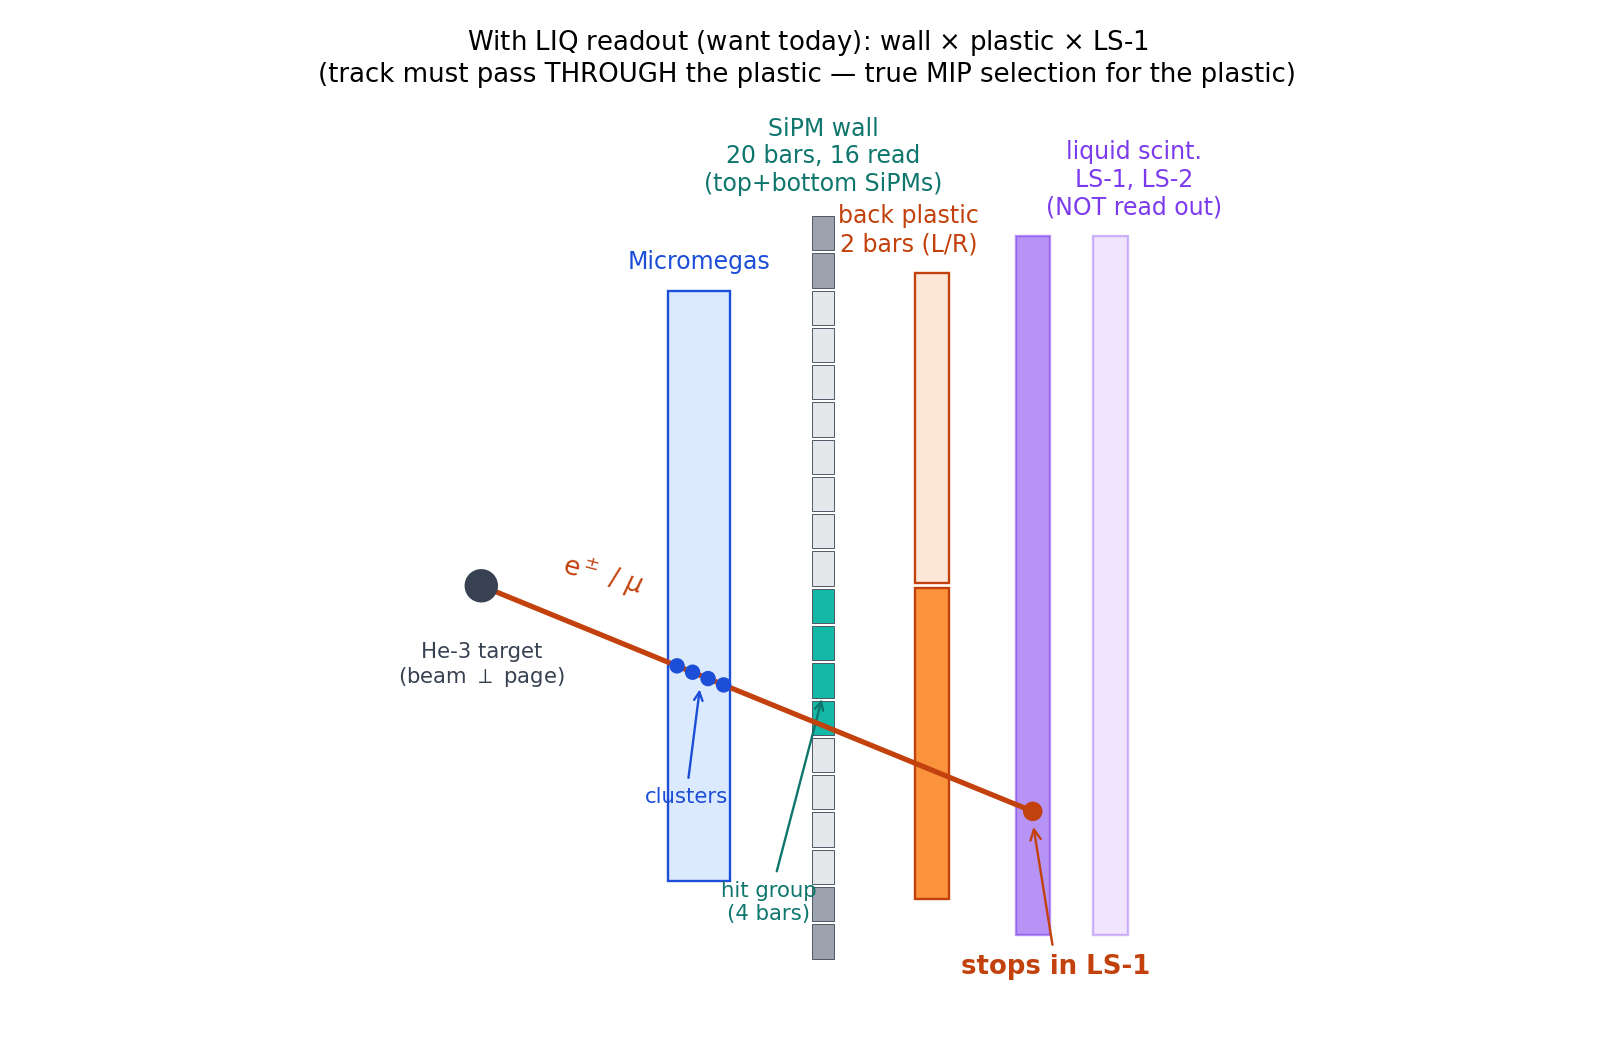
\includegraphics[width=\textwidth,height=.7\textheight,keepaspectratio]{11_diagrams/concept_wall_plastic_liq.png}

{\small Stack: MM $\to$ wall $\to$ plastic $\to$ LS. Wall$\times$plastic tags
wall MIPs only; adding a LIQ hit \emph{behind} the plastic selects
through-goers $\Rightarrow$ plastic spectrum in triples = plastic MIP
candidates. Double sideband subtraction in both dt's.}
\end{frame}

\begin{frame}{Result 4 --- the plastic MIP, found (PSSB2, one HV step per panel)}
\centering
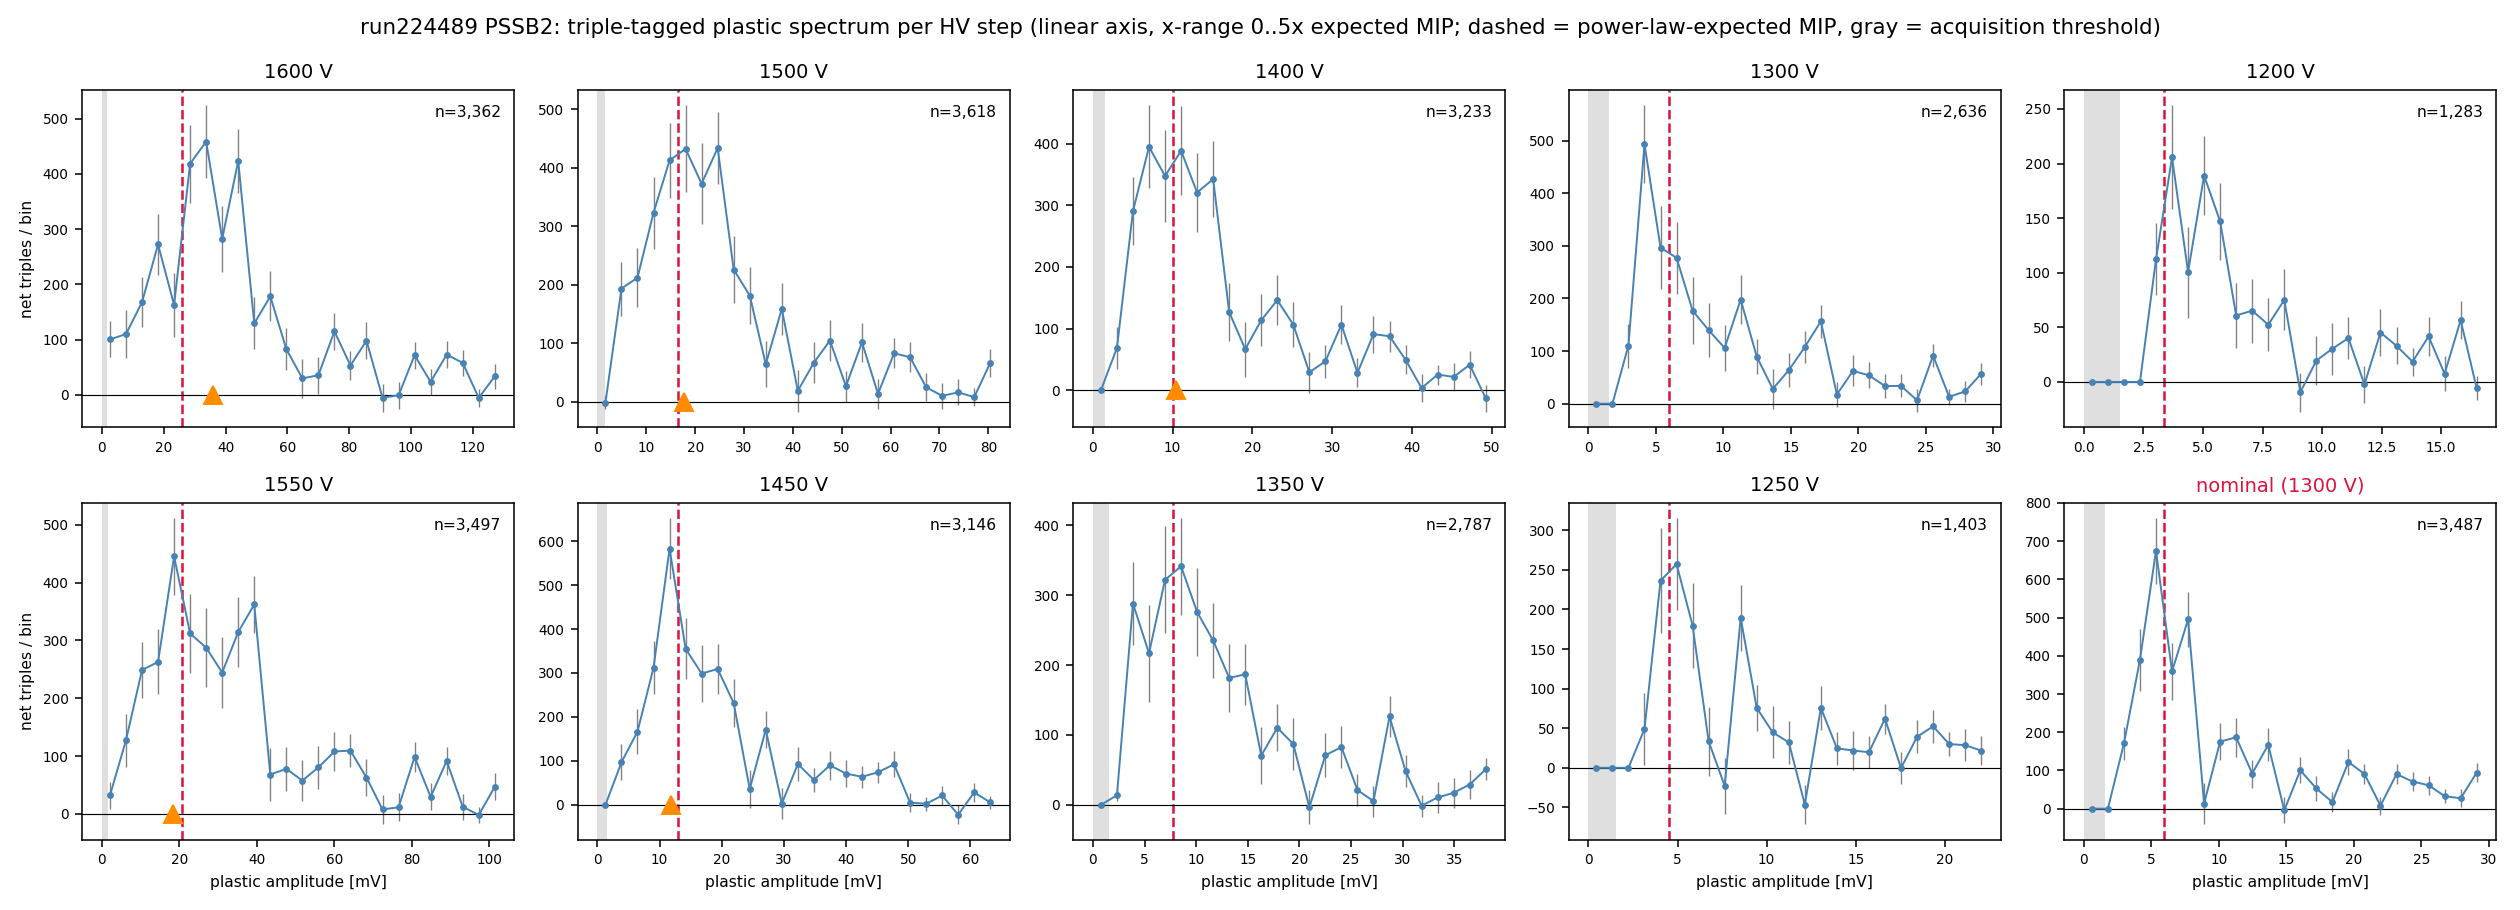
\includegraphics[width=\textwidth,height=.72\textheight,keepaspectratio]{19_triples/steps_linear/mip_steps_PSSB2.png}

{\small Linear amplitude axis, coarse bins, propagated Poisson errors. A
single significant peak tracks the power-law expectation (dashed) panel after
panel while the acquisition threshold (gray) stays put --- a threshold
artifact cannot do this. Orange: per-step fitted MPV. All 8 PMTs in
\texttt{figures/19\_triples/steps\_linear/}.}
\end{frame}

\begin{frame}{Weakest PMT (PSSD2): clear at high V, rides threshold at nominal}
\centering
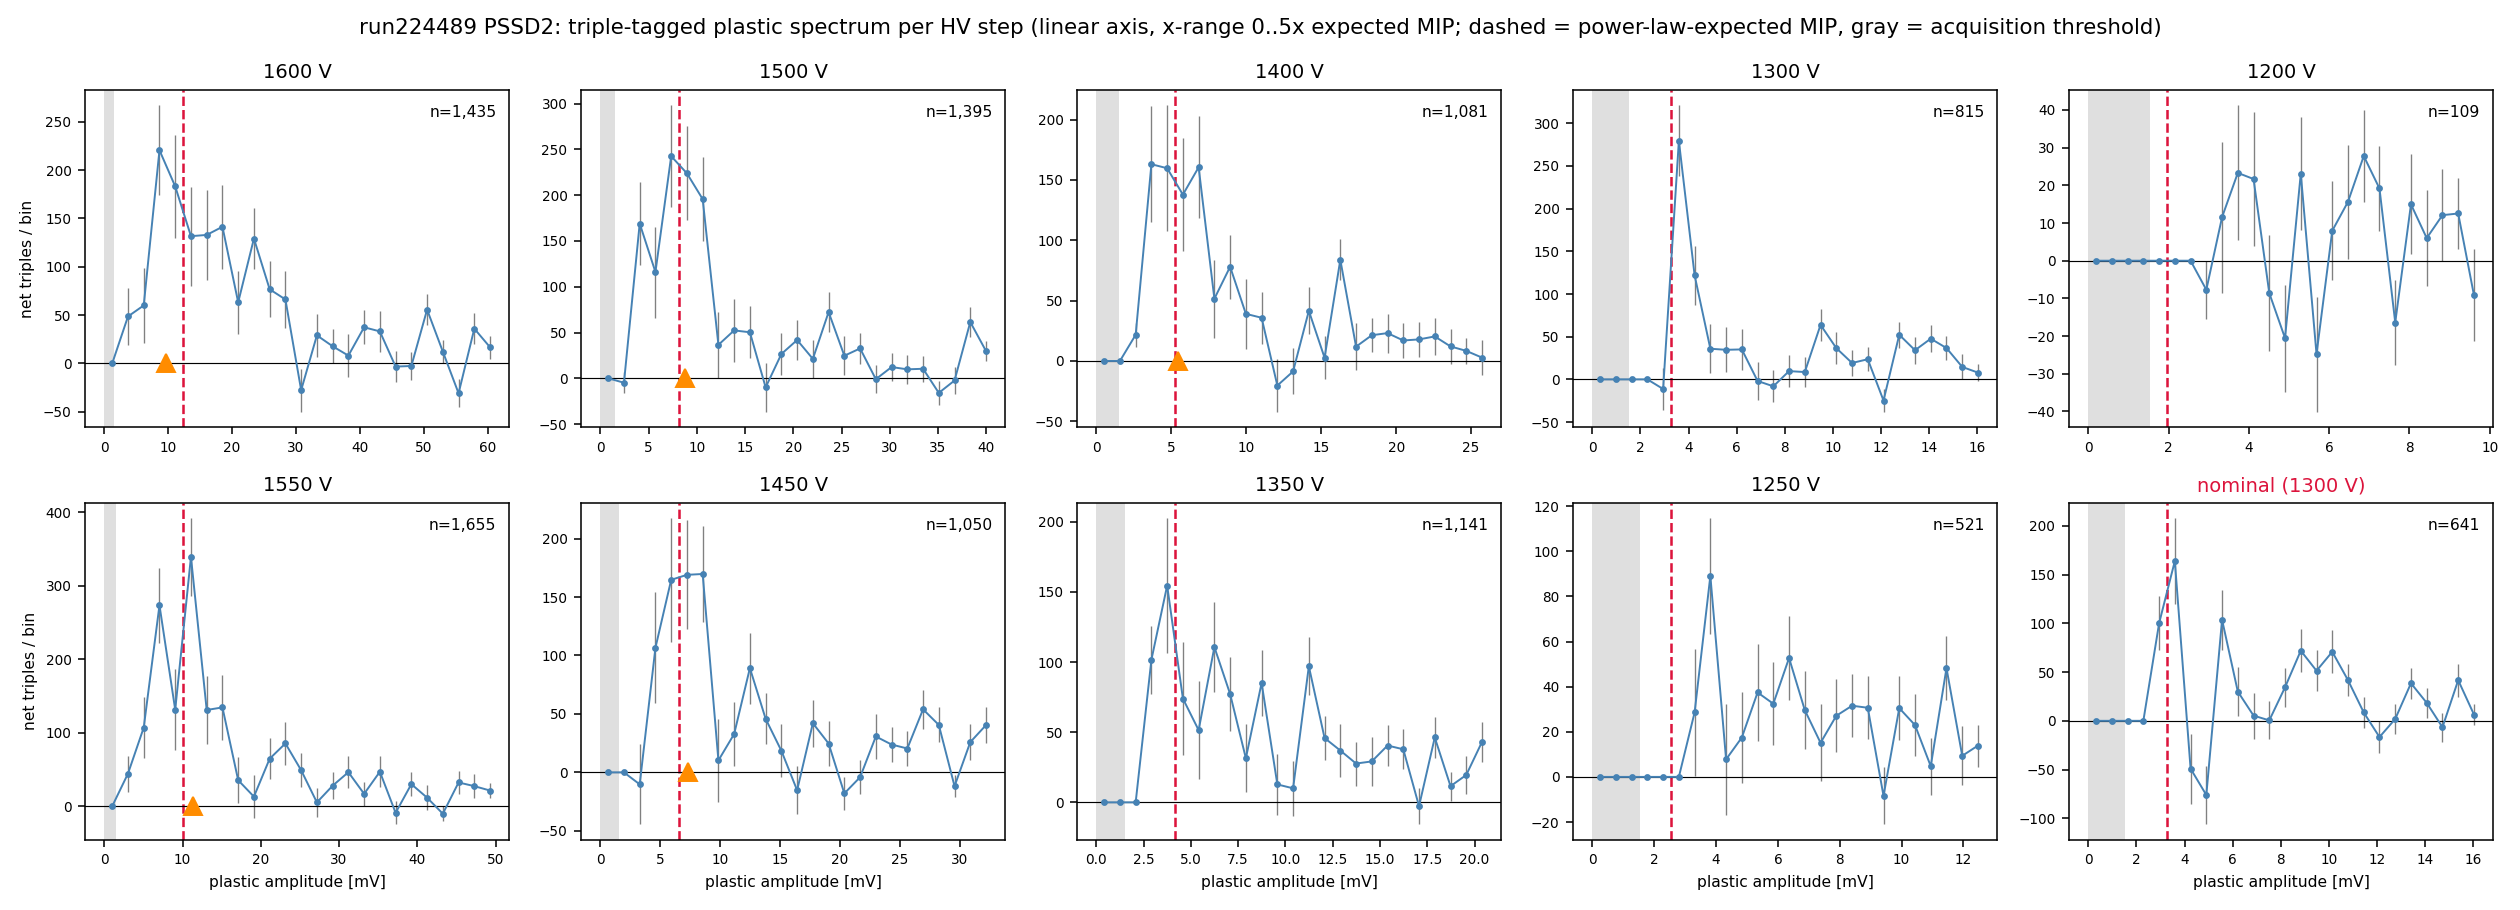
\includegraphics[width=\textwidth,height=.72\textheight,keepaspectratio]{19_triples/steps_linear/mip_steps_PSSD2.png}

{\small Peak clear of threshold only for $V\geq1400$ V $\Rightarrow$ only
those steps enter the fit; at nominal HV the DR MIP rides the threshold ---
this arm cannot trigger on plastic MIPs until equalized.}
\end{frame}

\begin{frame}{Cross-check: gain-aligned stack}
\centering
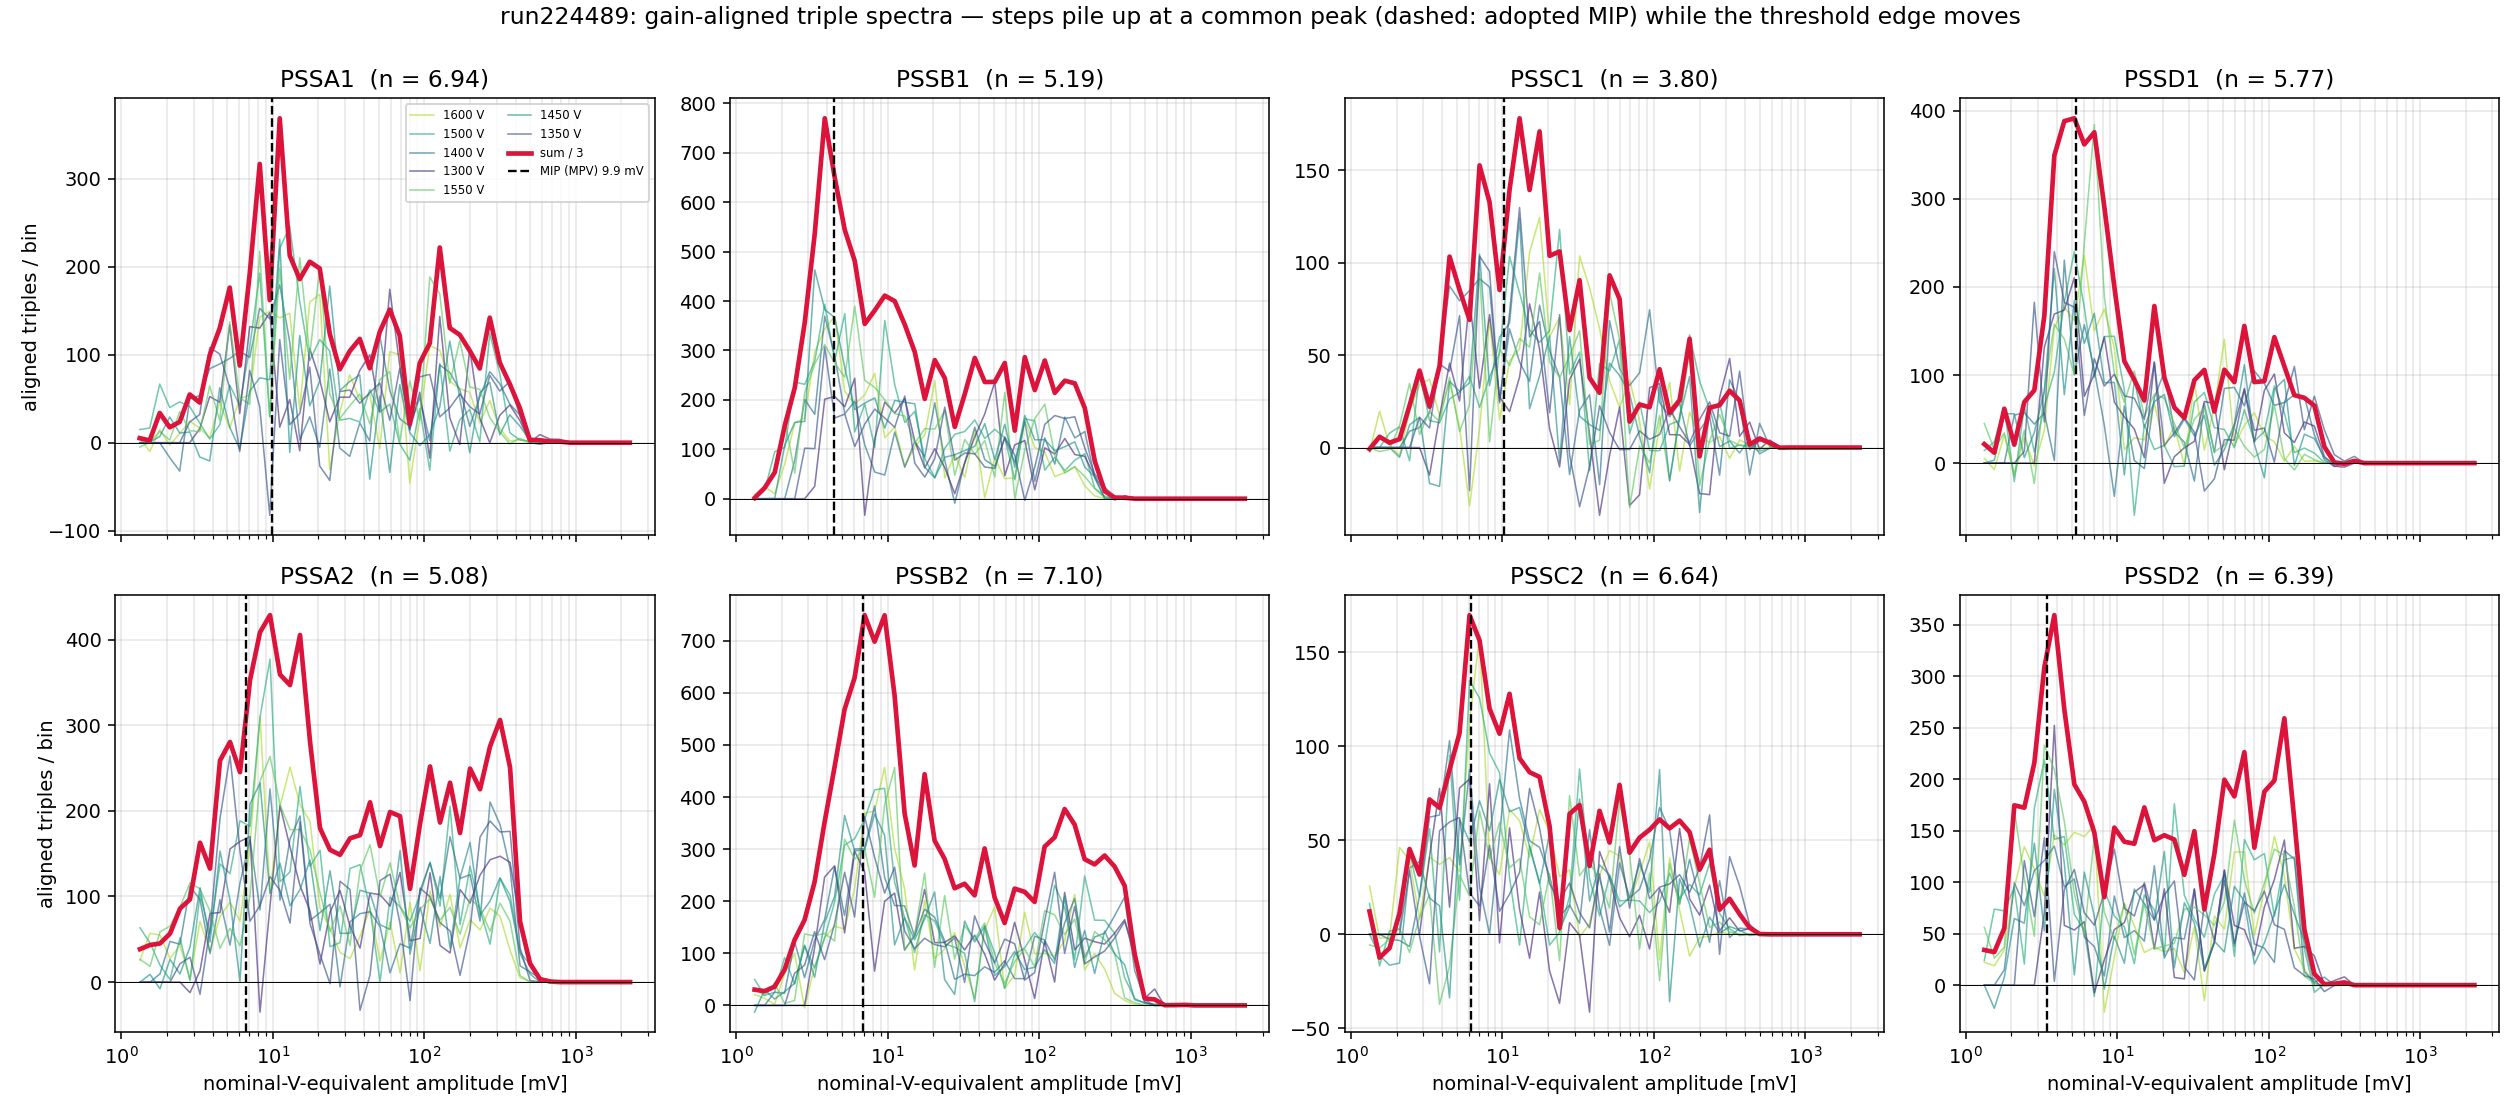
\includegraphics[width=\textwidth,height=.72\textheight,keepaspectratio]{19_triples/pss_mip_aligned.png}

{\small Each step's spectrum scaled to its nominal-V equivalent
($\times(V_{\rm nom}/V)^{n}$ = translation in log amp): the steps pile up at a
common peak and the sum (red) peaks at the adopted MPV (dashed) on every PMT.
(Log-amp representation --- peak positions here sit above the linear MPV.)}
\end{frame}

\begin{frame}{Trust check: MIP MPV vs the no-MIP-selection coincident median}
\centering
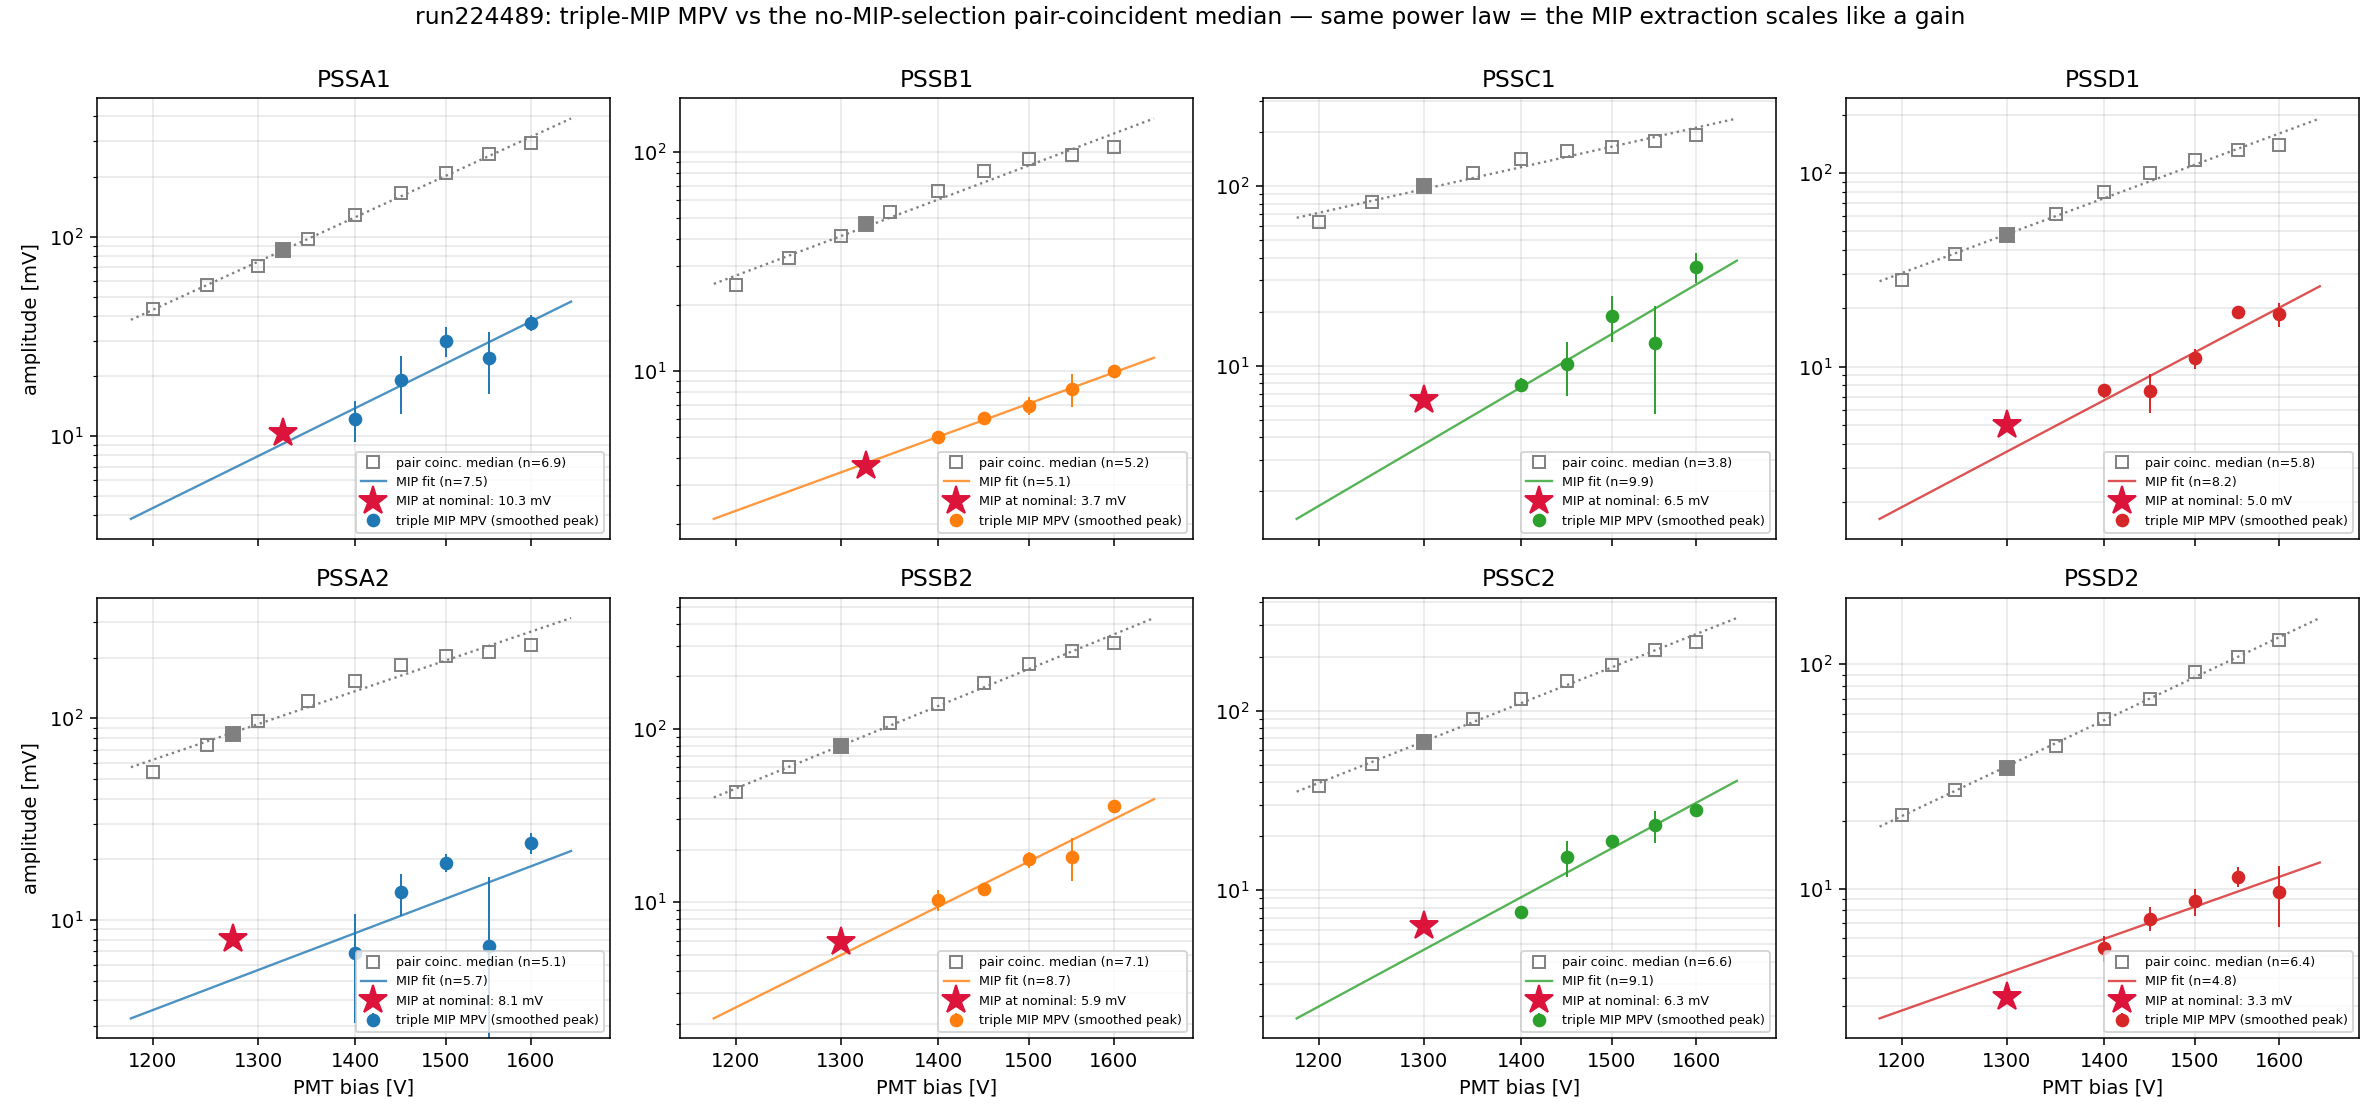
\includegraphics[width=\textwidth,height=.72\textheight,keepaspectratio]{19_triples/mip_vs_v_median_compare.png}

{\small Gray squares: pair-coincident median (no MIP selection,
$\sim$100$\times$ stats). Colored: per-step triple-MIP MPVs (bootstrap
errors) + own power-law fit. \textbf{Same slope, factor $\sim$10 below} ---
the MIP extraction scales like a gain; noise would not. Star: adopted
aligned-sum MPV at nominal.}
\end{frame}

\begin{frame}{First plastic-MIP calibration table (linear-space MPV)}
\begin{columns}
\column{.52\textwidth}
\centering\small
\begin{tabular}{lrrrr}
\toprule
PMT & MPV [mV] & spread & mV/MeV\\
\midrule
AL & $10.3\pm1.5$ & 16\% & 2.05\\
AR & $ 8.1\pm1.2$ & 42\%$^{*}$ & 1.60\\
BL & $ \alert{3.7}\pm0.5$ &  2\% & 0.73\\
BR & $ 5.9\pm0.5$ & 16\% & 1.18\\
CL & $ 6.5\pm1.6$ & 38\%$^{*}$ & 1.28\\
CR & $ 6.3\pm0.3$ & 18\% & 1.25\\
DL & $ 5.0\pm0.6$ & 18\% & 0.99\\
DR & $ \alert{3.3}\pm0.3$ & 14\% & 0.65\\
\bottomrule
\end{tabular}

{\scriptsize $^{*}$AR/CL genuinely less certain (per-step scatter). Energy
scale: 5.05 MeV in 2.5 cm PVT (normal incidence).}
\column{.45\textwidth}
\begin{itemize}
\item MPV = smoothed peak of the gain-aligned summed linear spectrum
      ($V\geq$1400 V steps); $\pm$ = Poisson bootstrap; spread = per-step
      transport scatter (the honest uncertainty on weak PMTs).
\item Linear-space MPV convention: first-pass log-binned modes were
      15--35\% high (mode of $dN/d\log A$ $\neq$ MPV of $dN/dA$).
\item Validated against the no-MIP-selection median (previous slide):
      same power law, factor $\sim$10 below.
\item \alert{DR (3.3 mV) and BL (3.7 mV) MPVs sit below the 4.9 mV
      trigger threshold} $\Rightarrow$ equalize before trusting plastic
      triggers on those arms.
\end{itemize}
\end{columns}
\end{frame}

\begin{frame}{Result 5 --- LIQ gain-vs-position gradient is \textbf{real}}
\centering
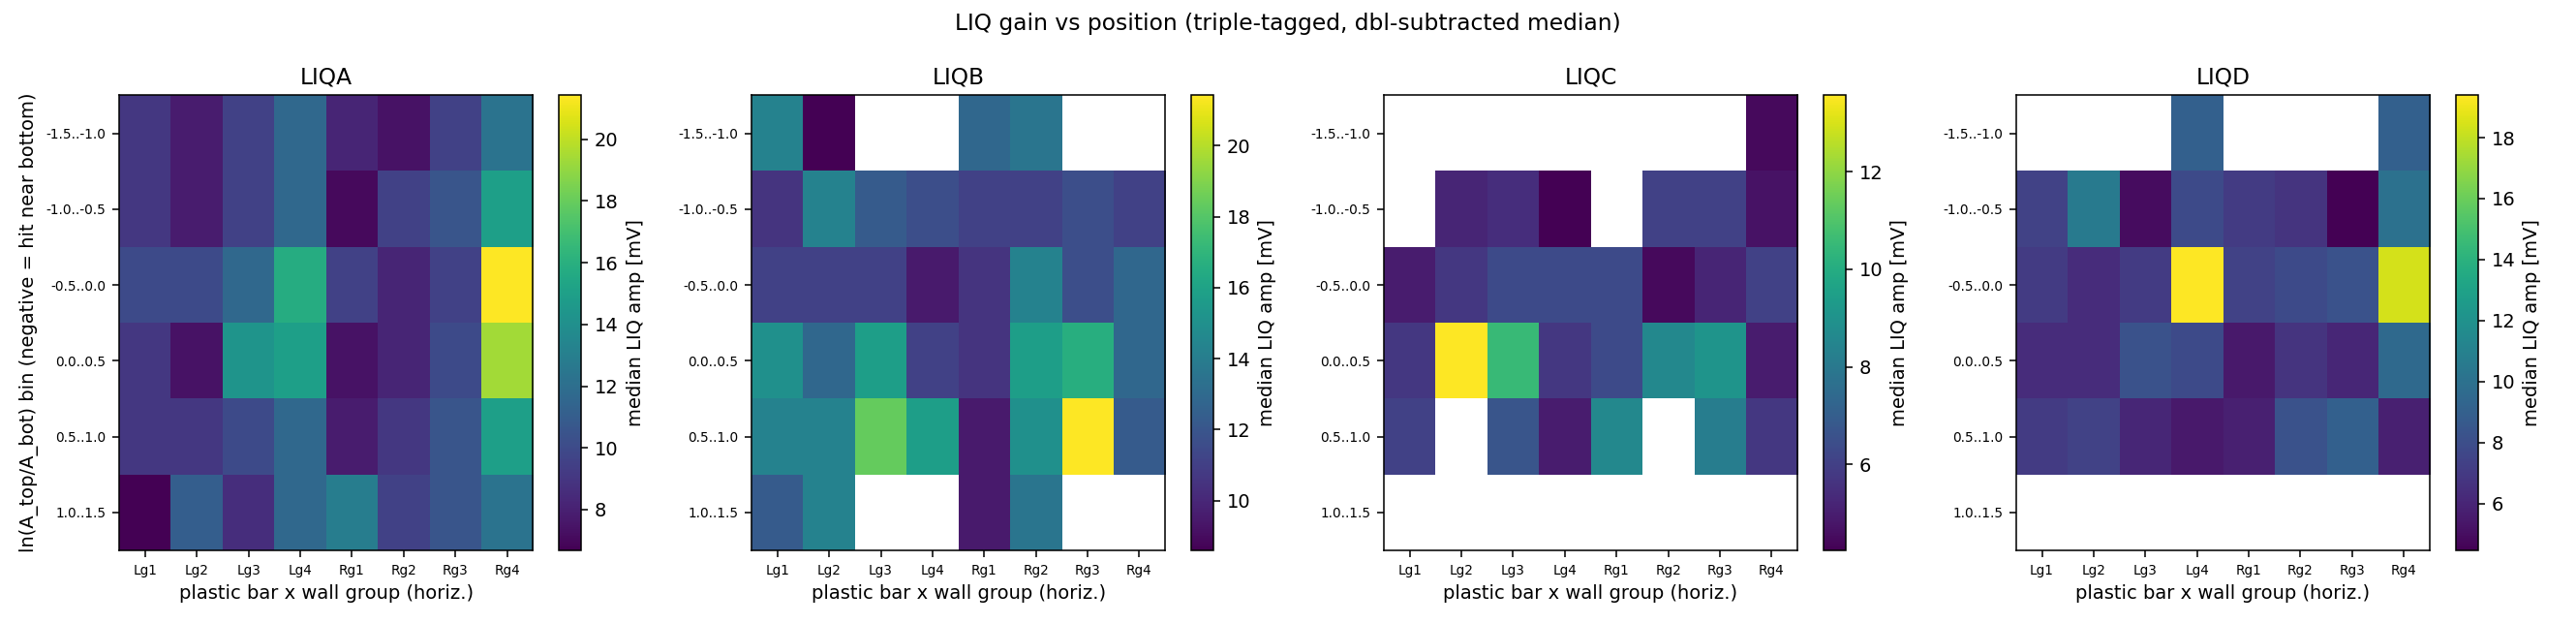
\includegraphics[width=\textwidth,height=.62\textheight,keepaspectratio]{19_triples/liq_position_map.png}

{\small Triple-tagged track position: horizontal = wall group $\times$ bar,
vertical = wall top/bottom asymmetry. 1.5--2$\times$ gradient toward the PMT;
axis flips with surveyed orientation: horizontal on A/D (PMT toward group 4),
vertical on B/C (PMT up) --- matches the as-built Geant geometry.}
\end{frame}

\begin{frame}{Timing: one clean common delay; the satellite misbehaves}
\begin{columns}
\column{.52\textwidth}
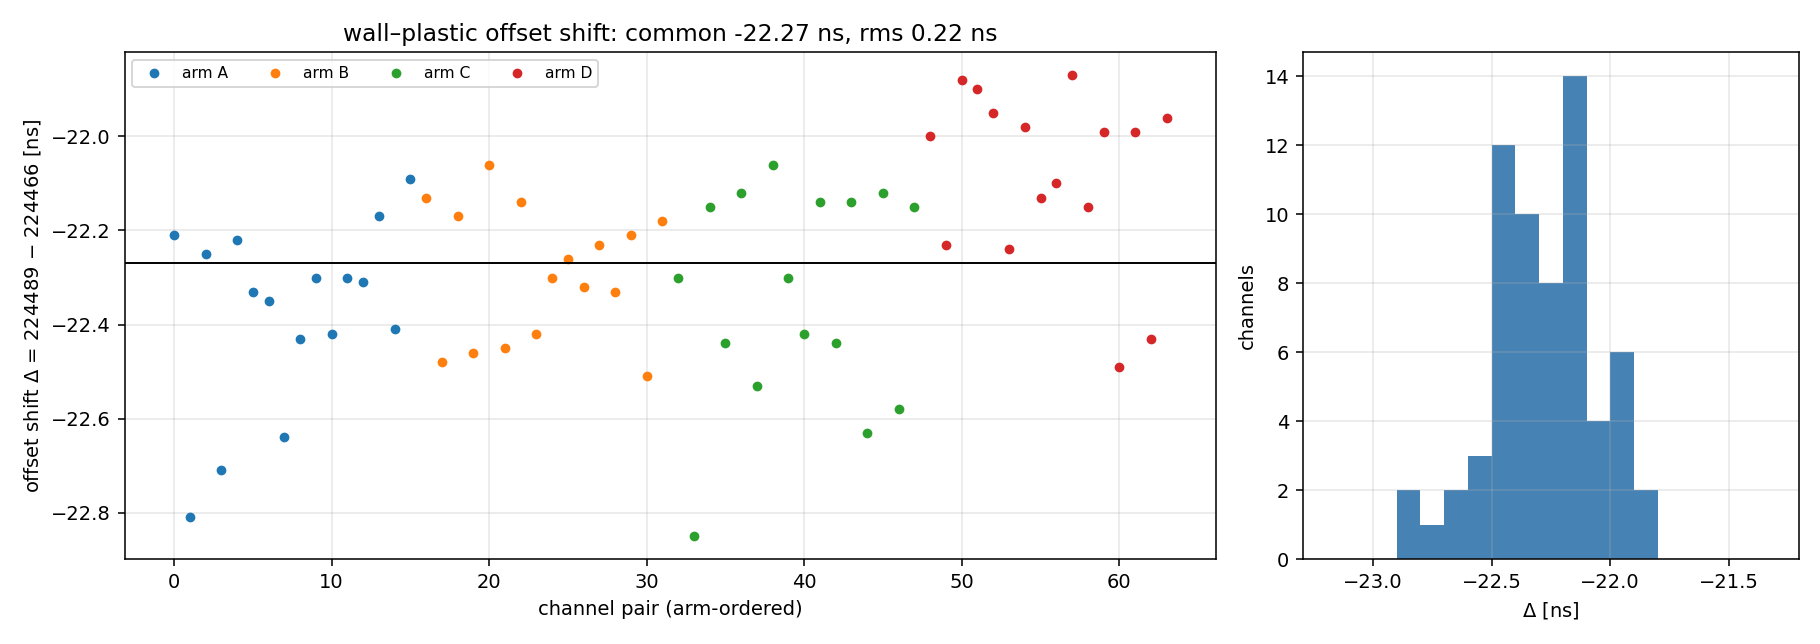
\includegraphics[width=\textwidth,height=.62\textheight,keepaspectratio]{19_triples/offset_shift.png}

{\small All 64 wall--plastic offsets shifted by a \textbf{common
$-22.27$ ns (rms 0.22 ns)}.}
\column{.46\textwidth}
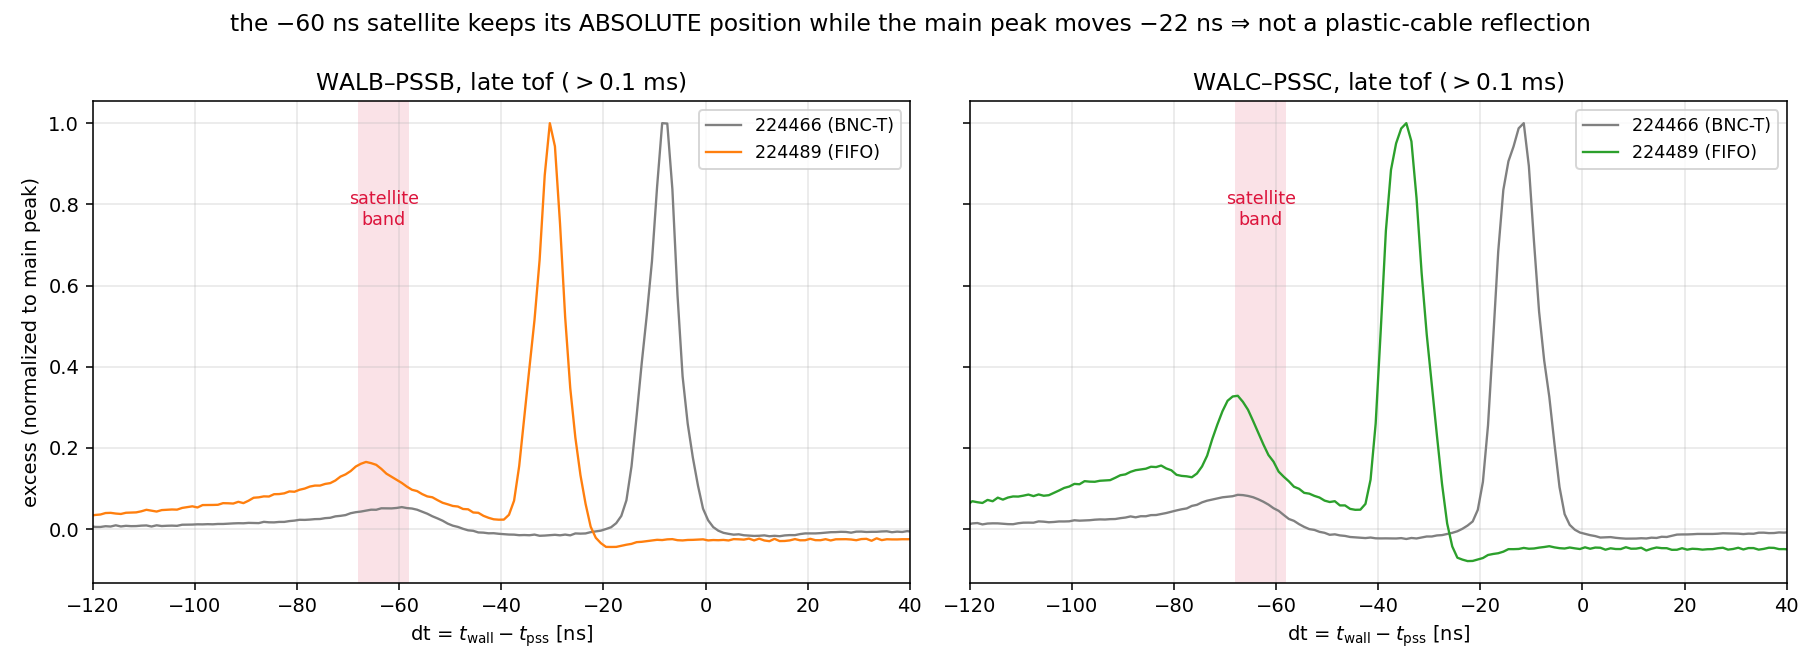
\includegraphics[width=\textwidth,height=.62\textheight,keepaspectratio]{19_triples/satellite.png}

{\small The $-60$ ns satellite kept its \emph{absolute} position (main peak
moved $-22$ ns) and grew to 19--34\% of the peak $\Rightarrow$ not a
plastic-cable reflection; injected at/after the FIFO. \alert{Scope check
recommended.} (Outside all analysis windows.)}
\end{columns}
\end{frame}

\begin{frame}{Summary}
\begin{enumerate}
\item \textbf{A/D cross-wiring fixed and confirmed} --- the old A/D deficit is
      fully explained; wall MIP calibration now covers all four arms.
\item \textbf{First plastic MIP calibration}: 0.65--2.05 mV/MeV at nominal HV
      via WAL$\times$PSS$\times$LIQ triples.
\item \textbf{FIFO ratio measured}: $\times$1.40 fleet (1.13--1.65 per PMT),
      not $\times$2.
\item \textbf{New HV equalization} ready (DAQ repo); apply it --- DR/BL cannot
      trigger on plastic MIPs at 4.9 mV until then.
\item \textbf{Liquids timed in}; LIQ position-gain gradient (1.5--2$\times$)
      confirmed and mapped; C/D LIQ gains look low --- review LIQ HV.
\item \textbf{Scope-check the FIFO} for the $-60$ ns satellite.
\end{enumerate}
\end{frame}

\begin{frame}{Backup: per-step triple spectra (low stats per step)}
\centering
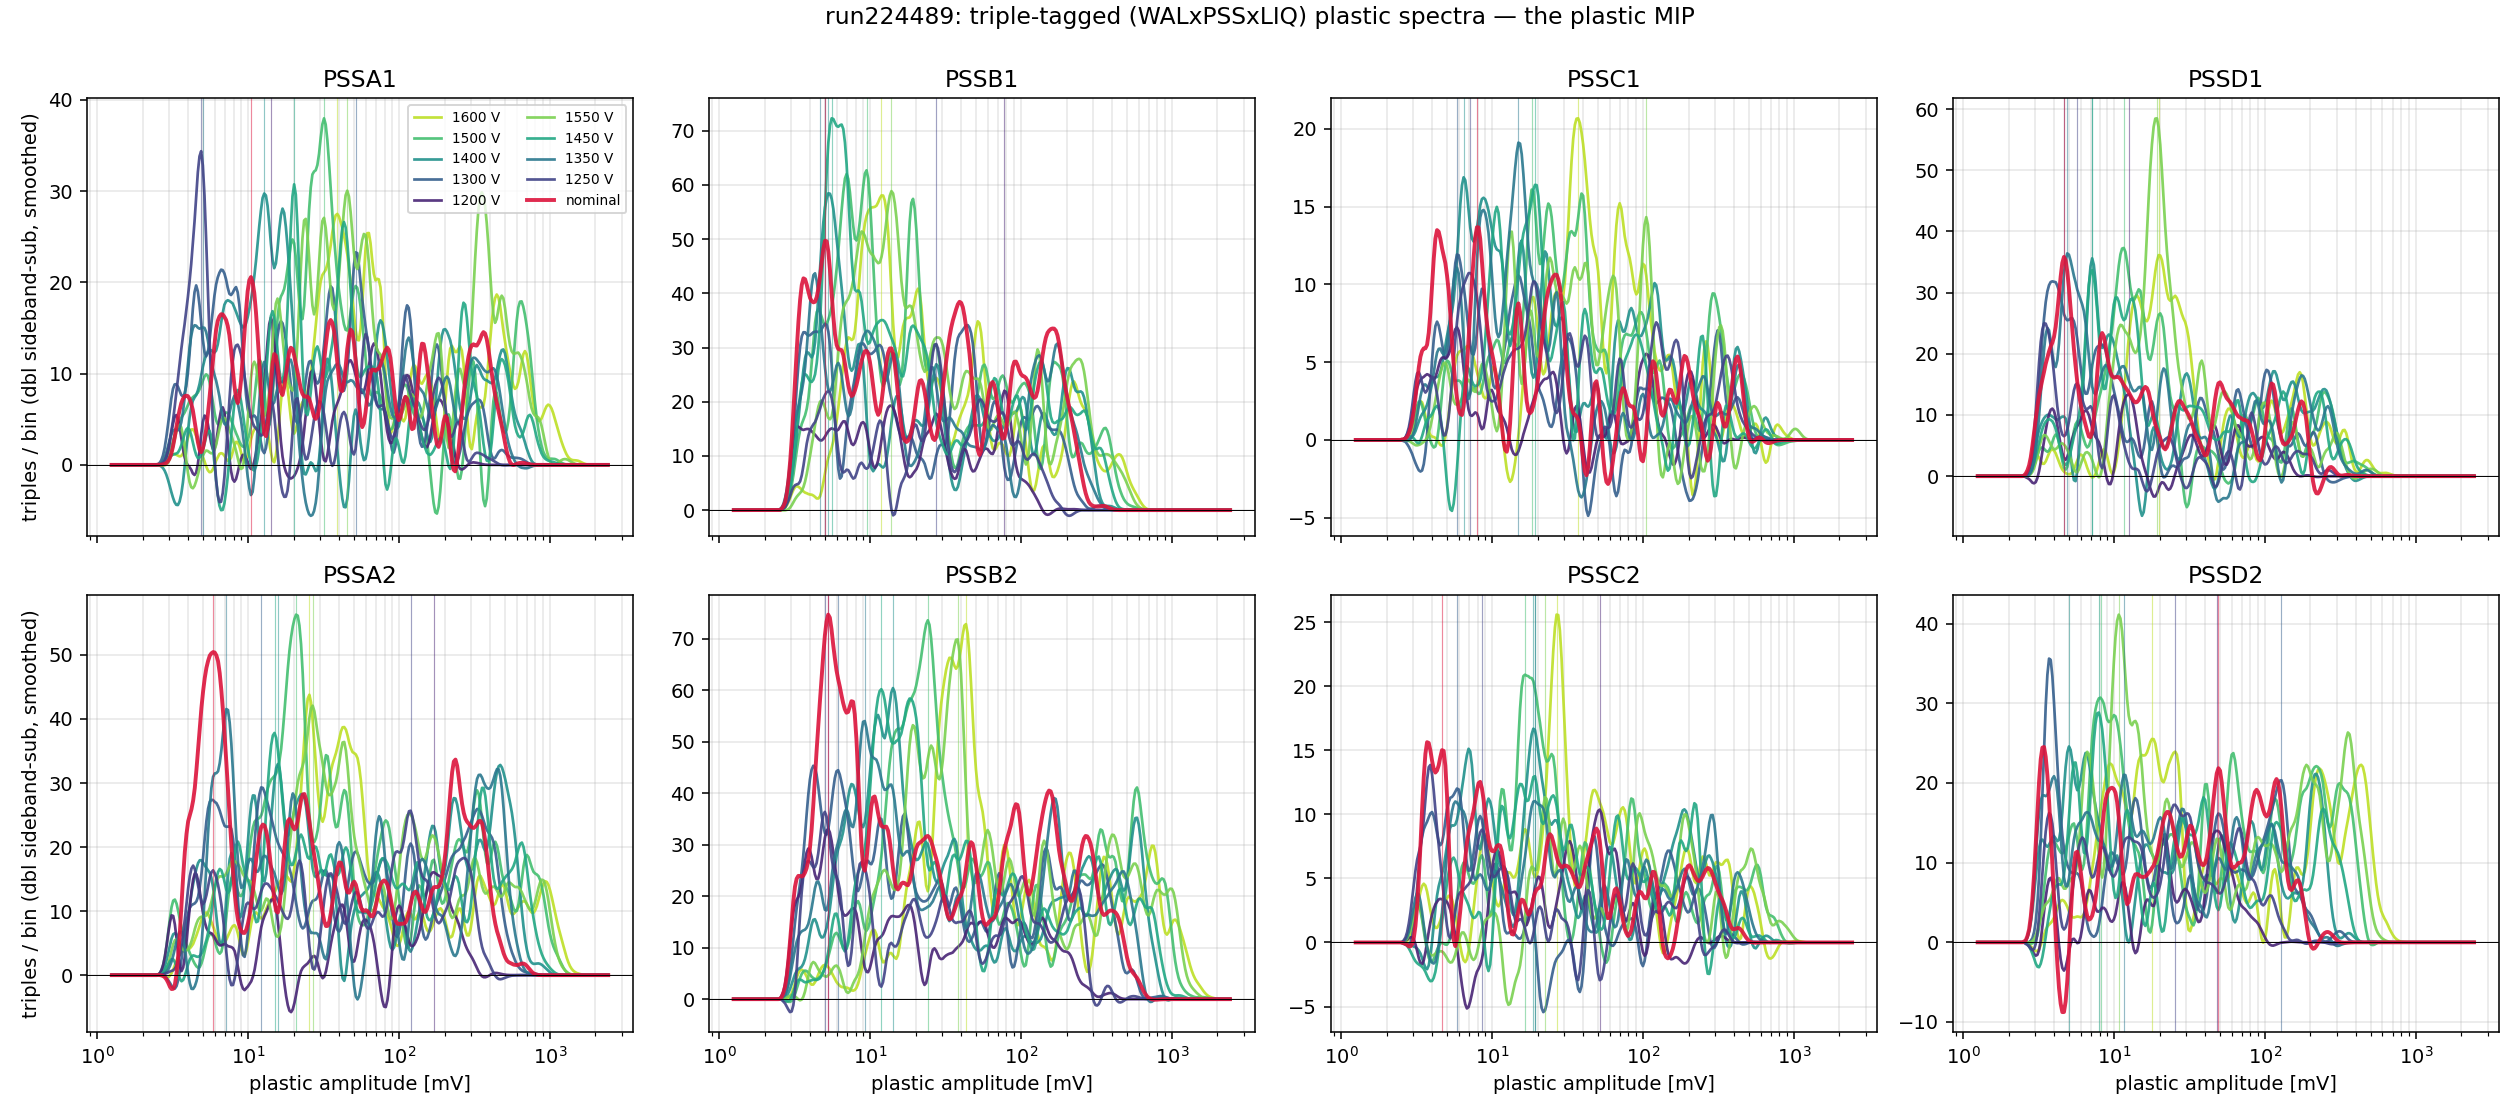
\includegraphics[width=\textwidth,height=.72\textheight,keepaspectratio]{19_triples/pss_mip_spectra.png}

{\small $\sim$2--6 k net triples per PMT per step after double sideband
subtraction --- individually noisy; the gain-aligned stack is the evidence
plot, these show the raw marching with HV.}
\end{frame}

\begin{frame}{Backup: wall spectrum unchanged by the LIQ tag}
\centering
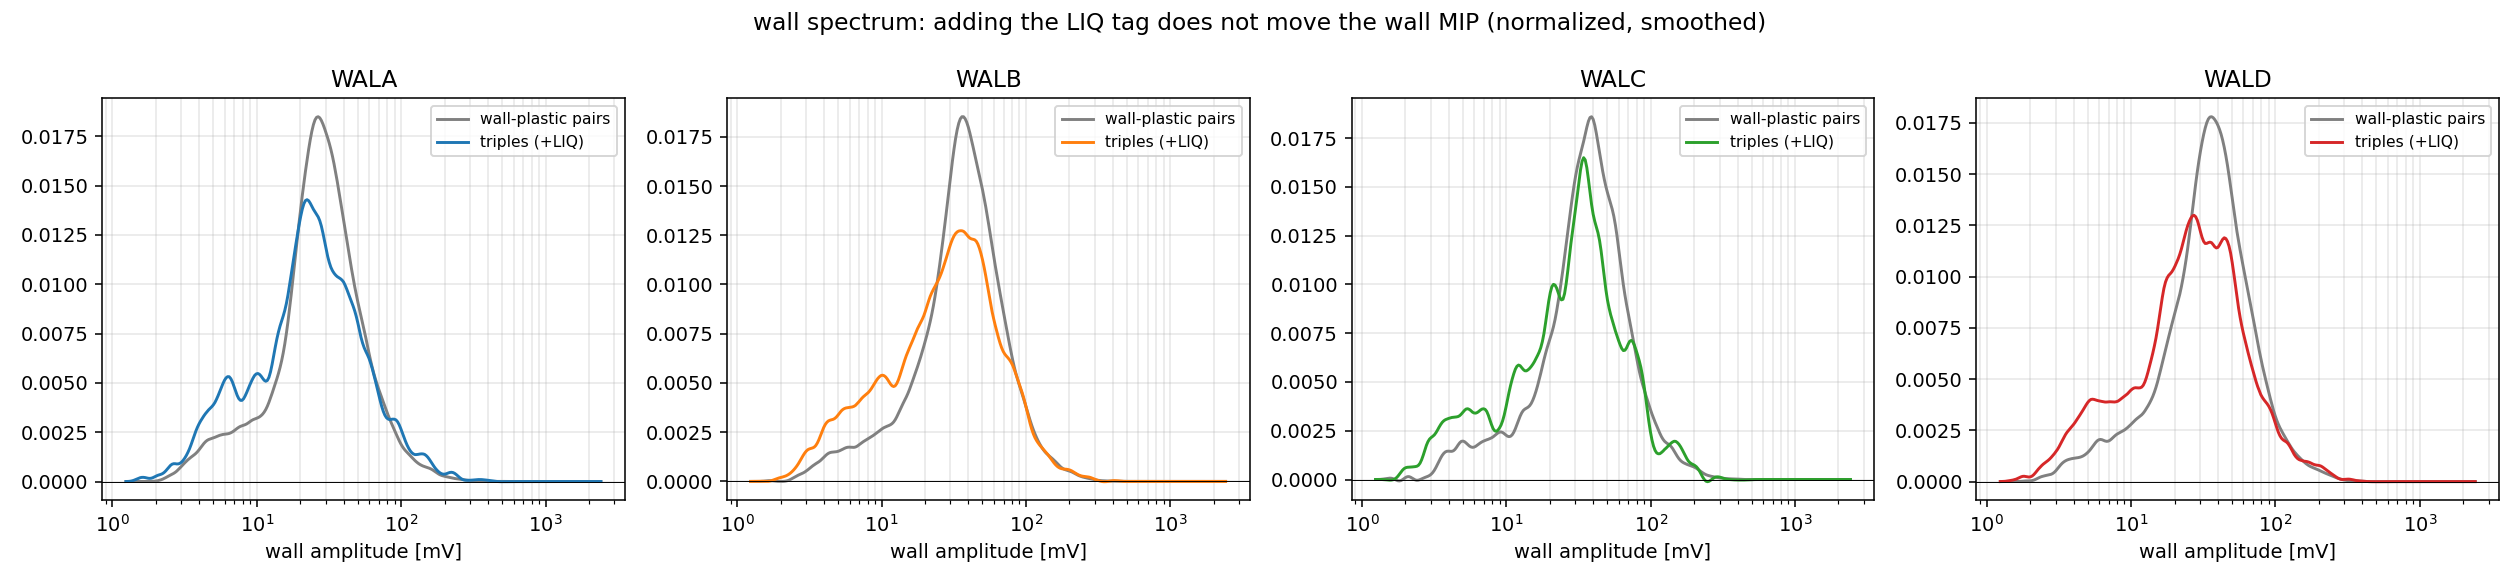
\includegraphics[width=\textwidth,height=.78\textheight,keepaspectratio]{19_triples/wall_in_triples.png}
\end{frame}

\begin{frame}{Backup: triple-tagged LIQ spectra (C/D low)}
\centering
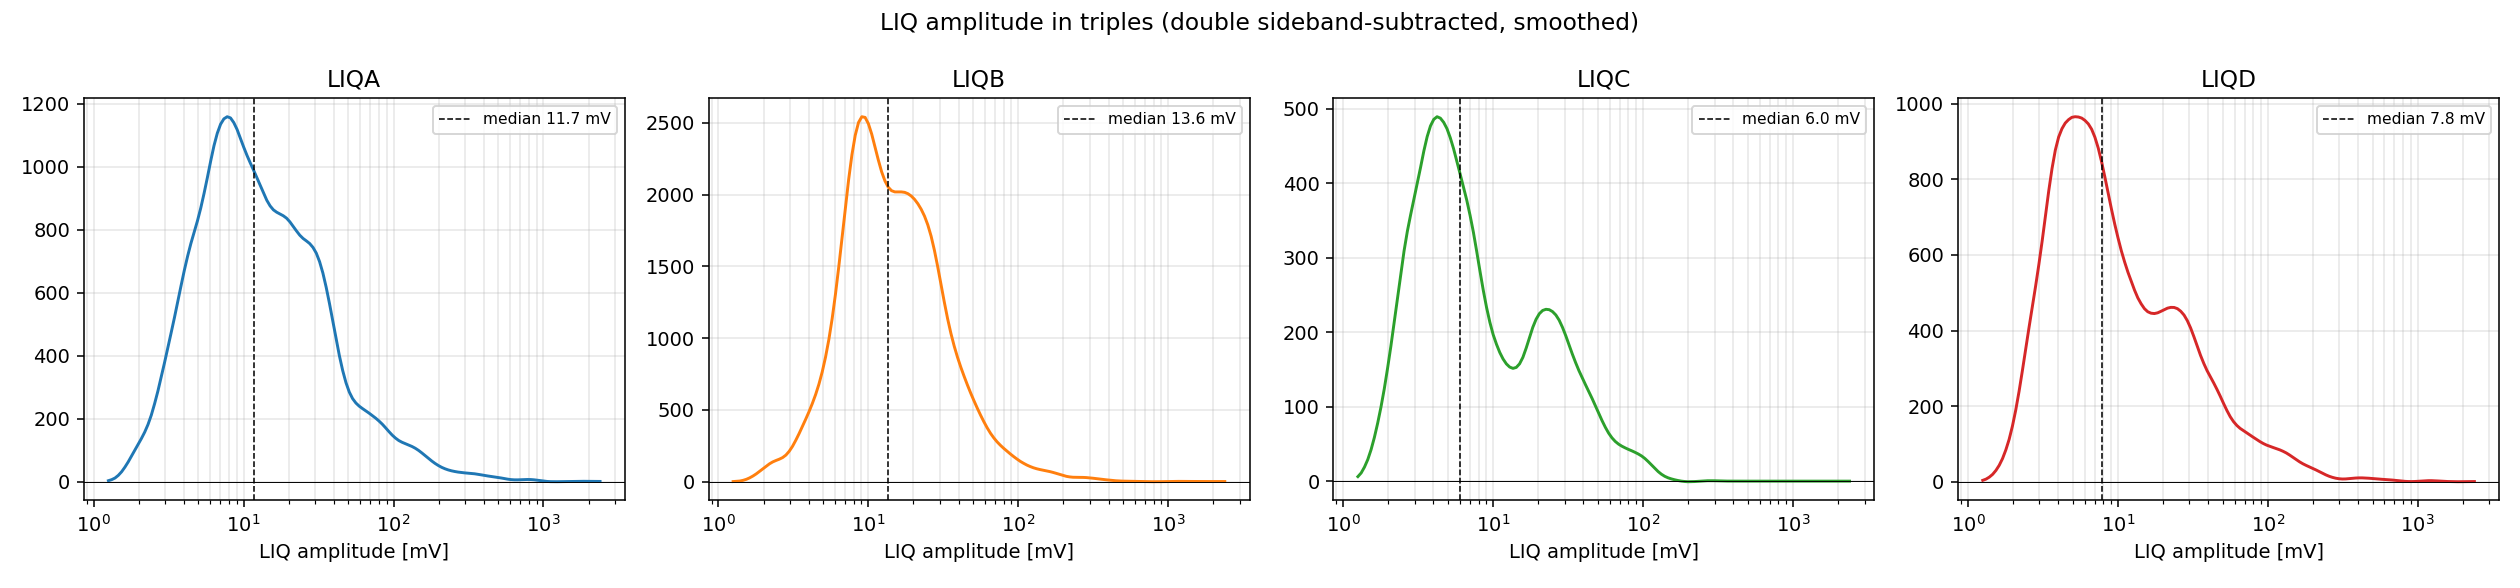
\includegraphics[width=\textwidth,height=.7\textheight,keepaspectratio]{19_triples/liq_spectra.png}

{\small Inclusive LIQ medians: A 7.5, B 10.4, C 4.7, D 5.3 mV.}
\end{frame}

\begin{frame}{Backup: coincident spectra per step (linear mV)}
\centering
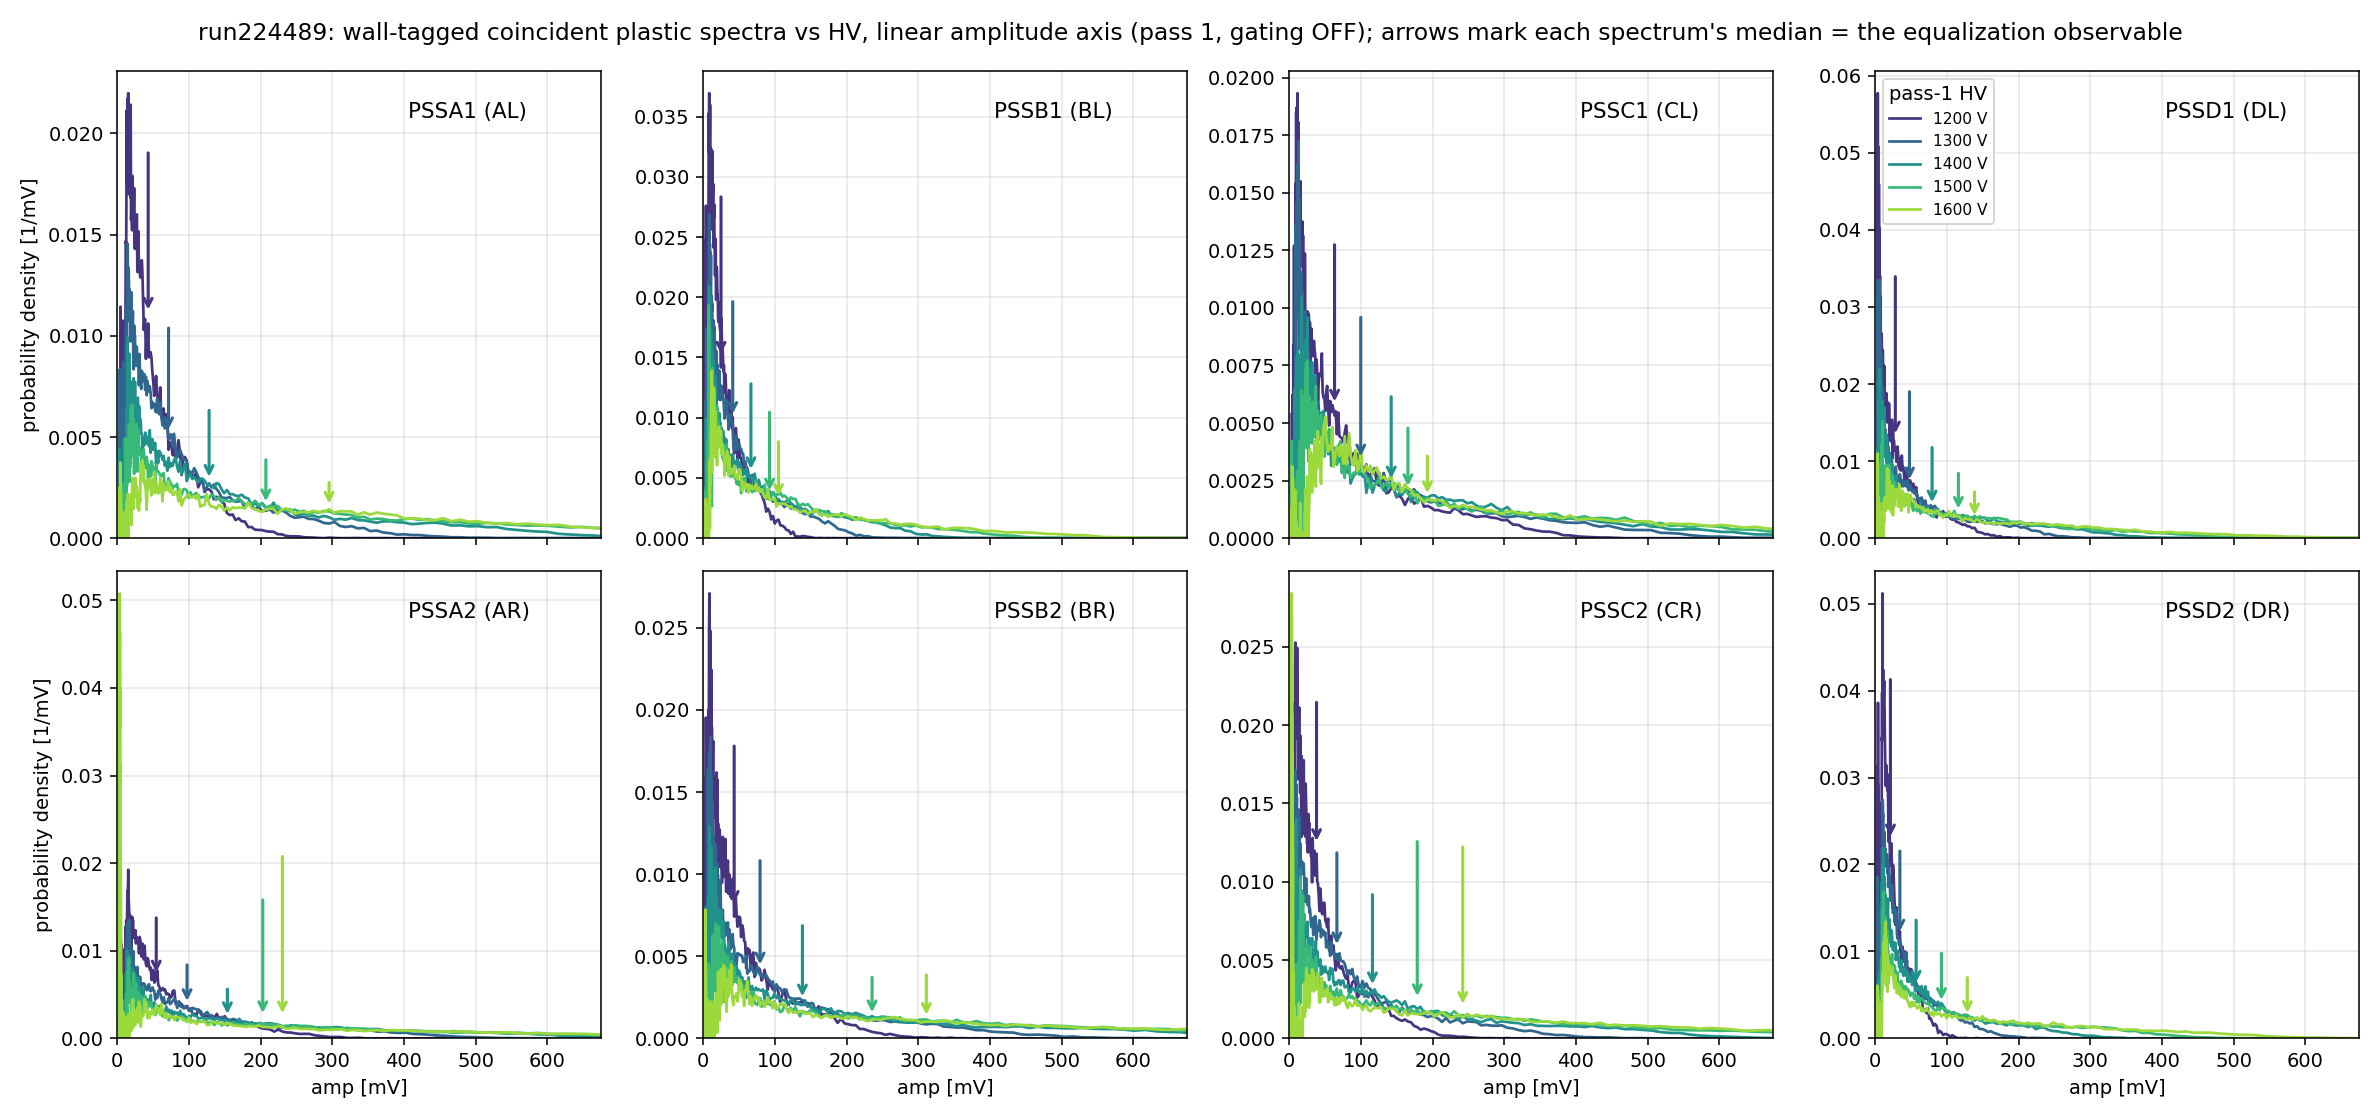
\includegraphics[width=\textwidth,height=.78\textheight,keepaspectratio]{12_hv_scan/coinc_spectra_linear.png}
\end{frame}

\begin{frame}{Backup: trigger threshold scan at equalized gains}
\centering
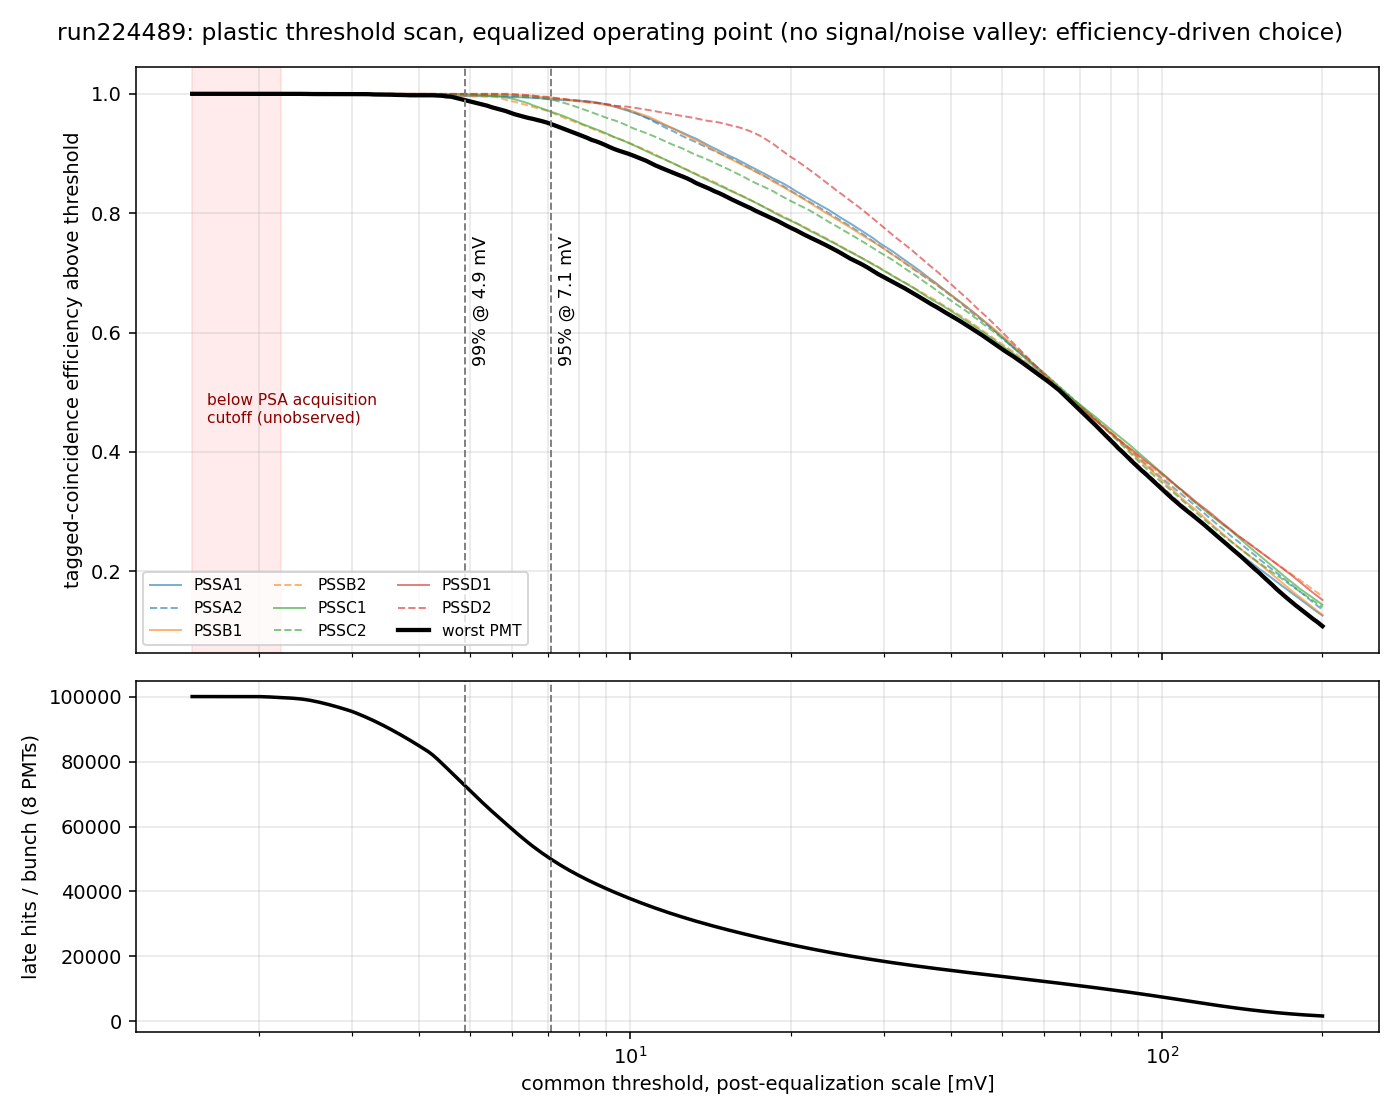
\includegraphics[width=\textwidth,height=.78\textheight,keepaspectratio]{12_hv_scan/threshold_scan.png}
\end{frame}

\end{document}
